\chapter{Phase III - analyse}

Différents types d'endpoint sont possibles :
\begin{enumerate}
    \item Endpoint continu
    \item Endpoint discret
    \item Endpoint de survie
\end{enumerate}

\section{Endpoint continu}
Pour chaque patient, on mesure un endpoint continu dont on va en général supposer qu’il suit une distribution approximativement normale. Par exemple, le Taux de cholestérol, Valeur de la pression artérielle, etc.\\

Si on peut supposer que notre endpoint suit une distribution normale, on va en général s’intéresser à la moyenne de cette distribution pour chaque bras de traitement

\subsection{Cas de deux groupes de traitements}

on considère deux groupes de traitement.
\begin{figure}[H]
    \centering
    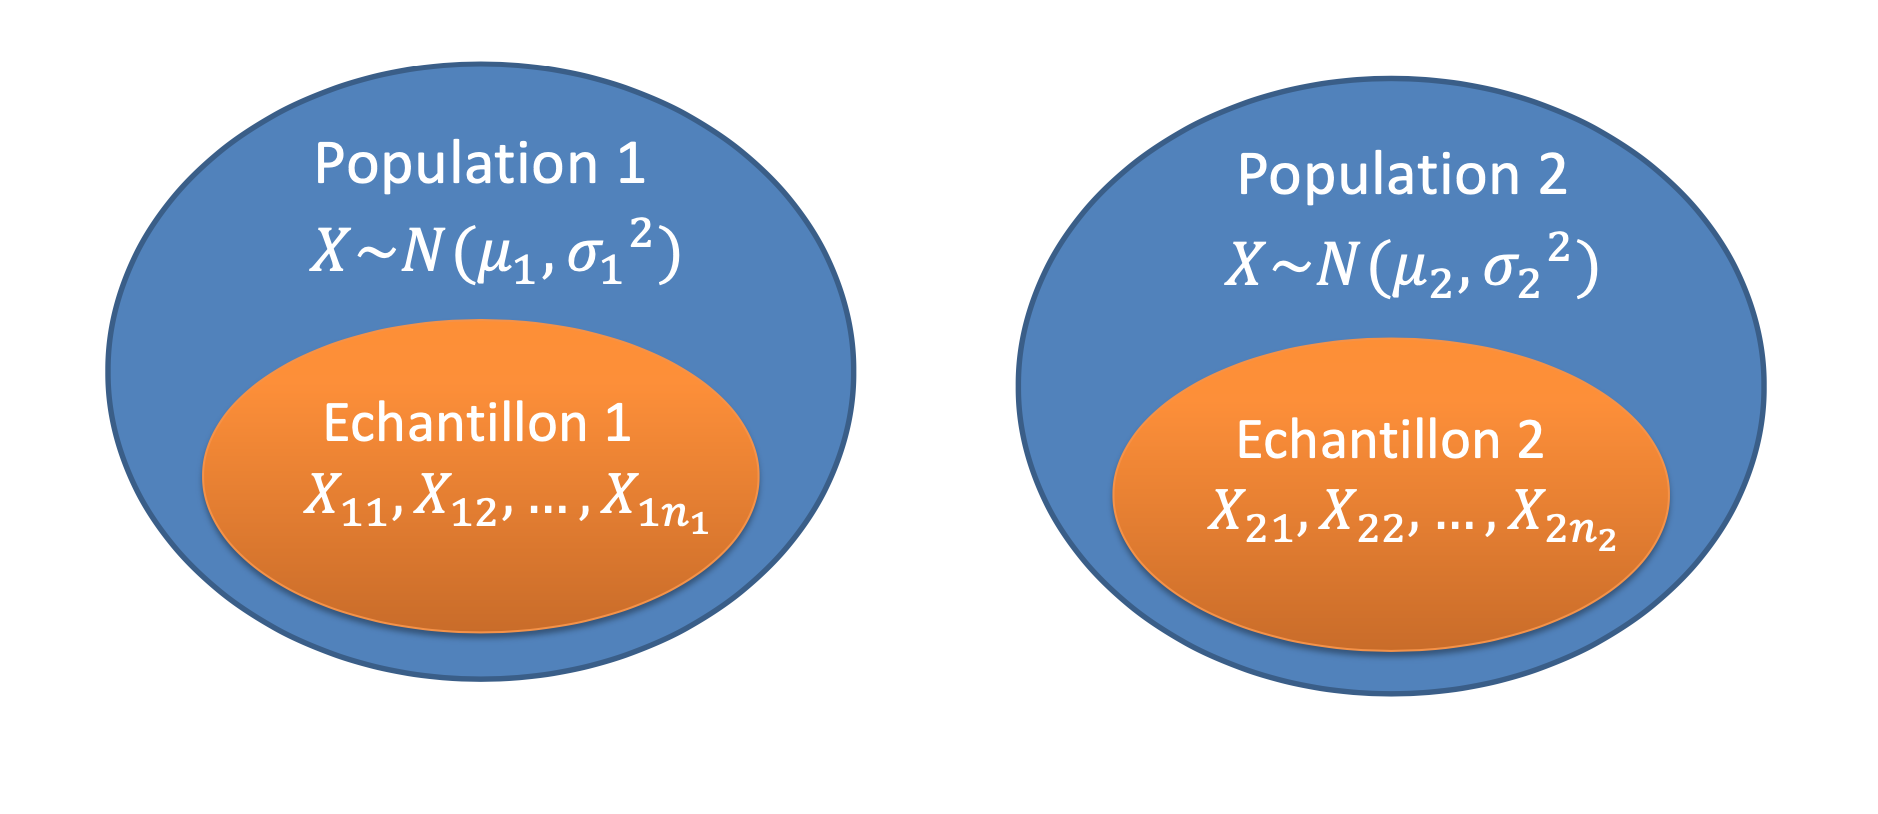
\includegraphics[scale = 0.5]{images/2groupescontinu.png}
    \caption{deux groupes de traitement}
    \label{fig:my_label}
\end{figure}




Test t de Student pour comparer deux moyennes :
\begin{figure}[H]
    \centering
    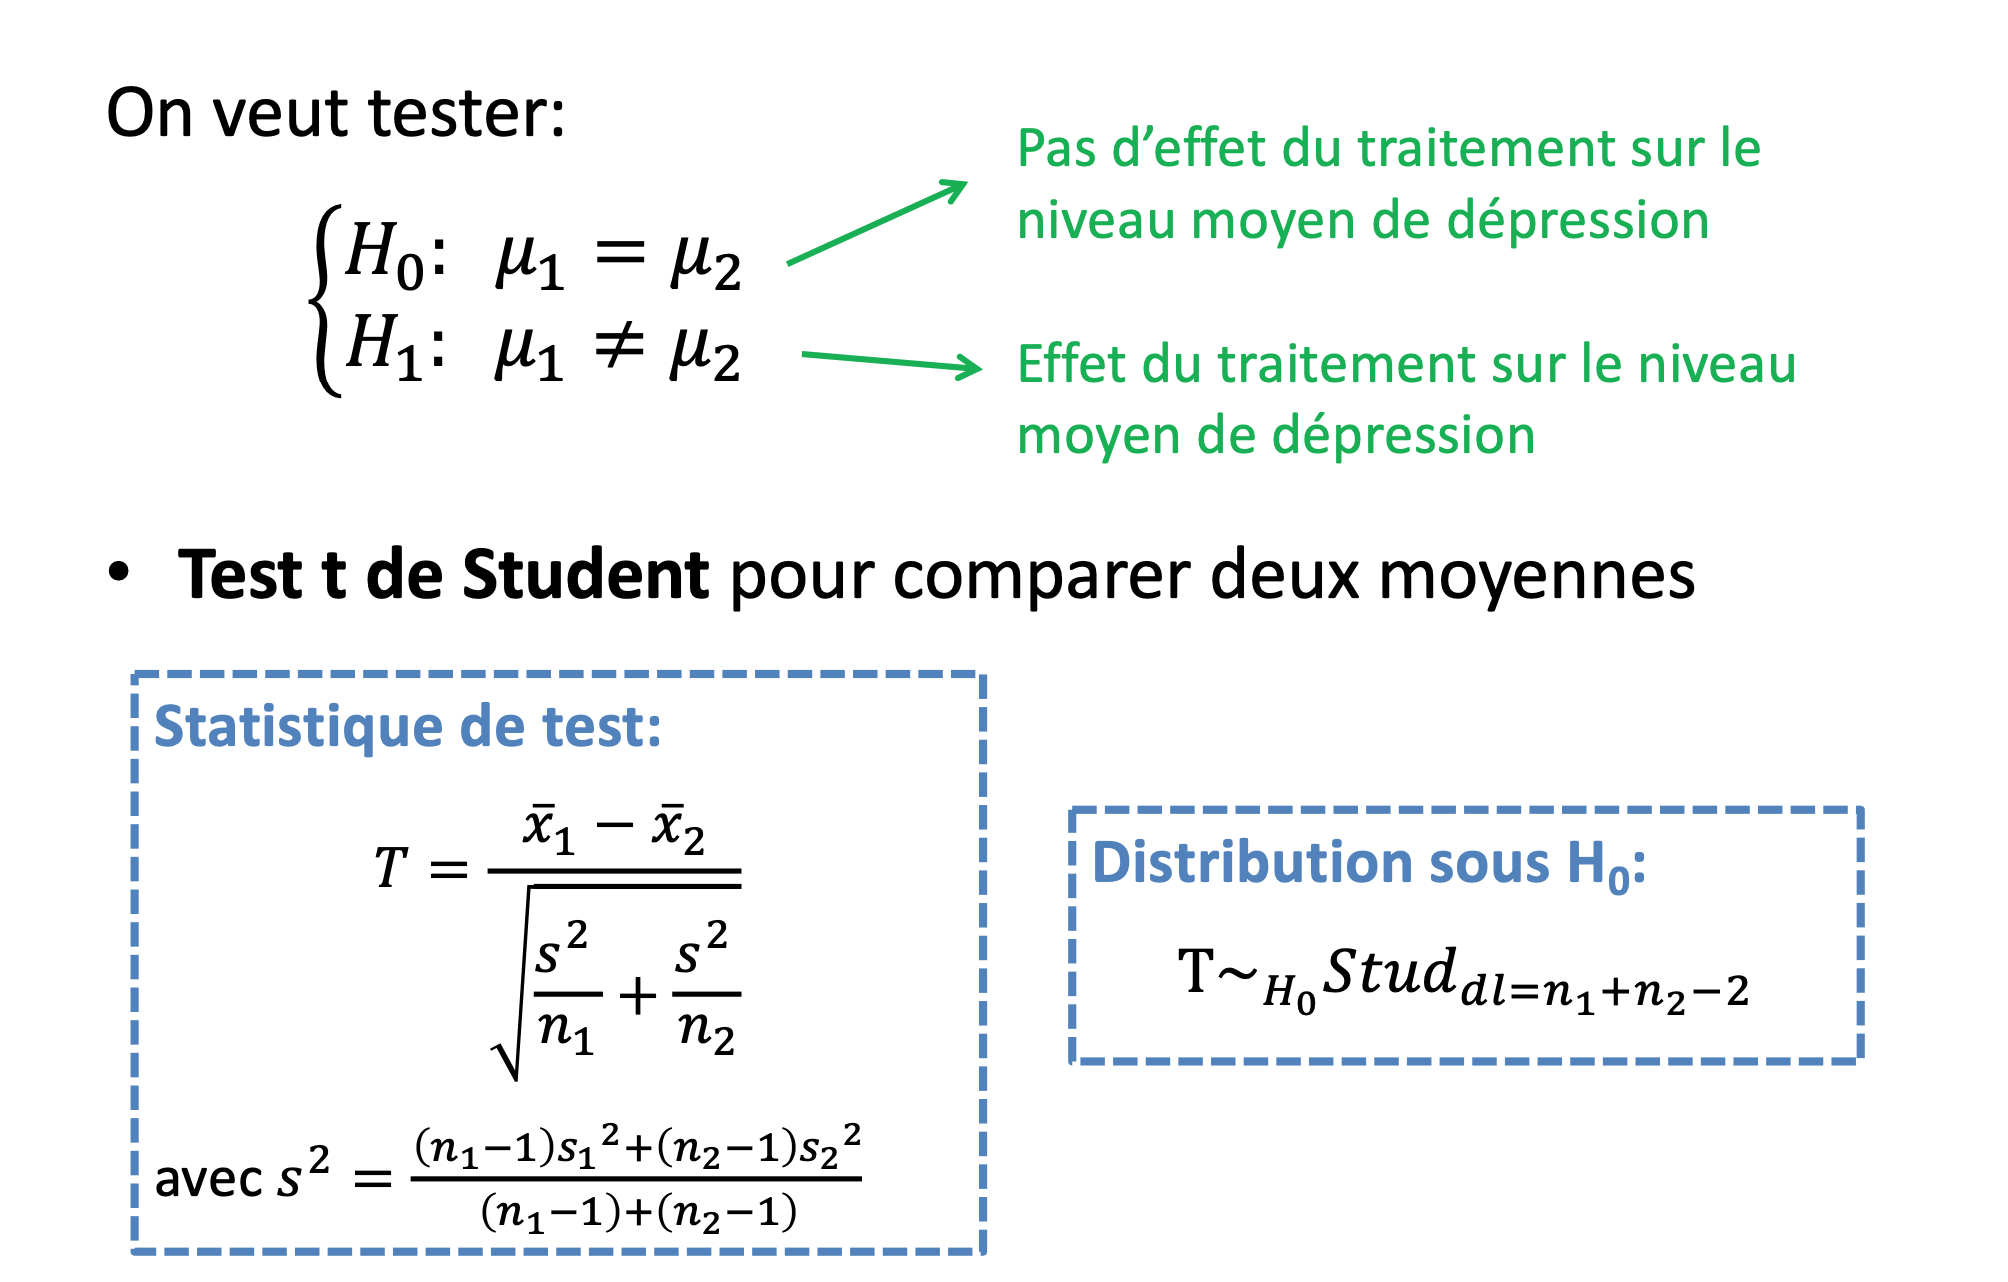
\includegraphics[scale=0.3]{images/student.png}
    \caption{Test t de Student pour comparer deux moyennes}
    \label{fig:my_label}
\end{figure}


\textbf{Remarques}
\begin{enumerate}
    \item \textbf{Conditions d’applications du test t de Student:}
    \begin{itemize}
        \item X est une variable continue de distribution (approximativement) normale, et de même variance dans les deux sous-populations considérées
        \item Les deux échantillons(aléatoires) sont indépendants
    \end{itemize}
    \item Si on ne peut pas supposer $\sigma_{1}^{2}=\sigma_{2}^{2}$, il existe une autre formulation de ce test
    
    \item Test de Welch: dans le cas où on ne peut supposer $\sigma_{1}^{2}=\sigma_{2}^{2}$, une meilleure approximation de la distribution sous H0 est donnée dans la figure \ref{fig:welch}
    \item Si on ne peut pas supposer la normalité approximative :
    \begin{itemize}
        \item On peut essayer de transformer la variable X, par exemple en considérant log(X), pour améliorer l’approximation normale
        \item On peut réaliser un test non paramétrique : Mann-Whitney-Wilcoxon U-test


    \end{itemize}
\end{enumerate}

\begin{figure}[H]
    \centering
    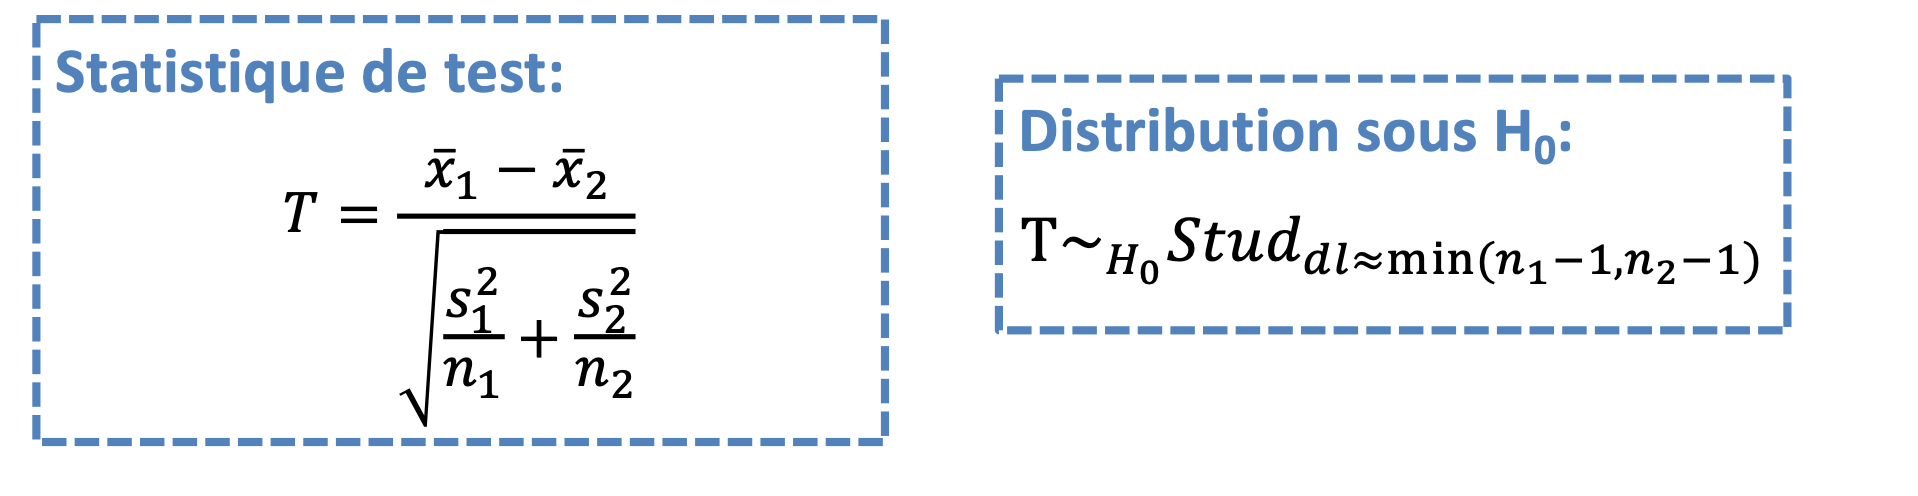
\includegraphics[scale = 0.5]{images/studentbis.png}
    \caption{Test t de Student pour comparer deux moyennes si $\sigma_{1}^{2} \neq \sigma_{2}^{2}$}
    \label{fig:studbis}
\end{figure}

\begin{figure}[H]
    \centering
    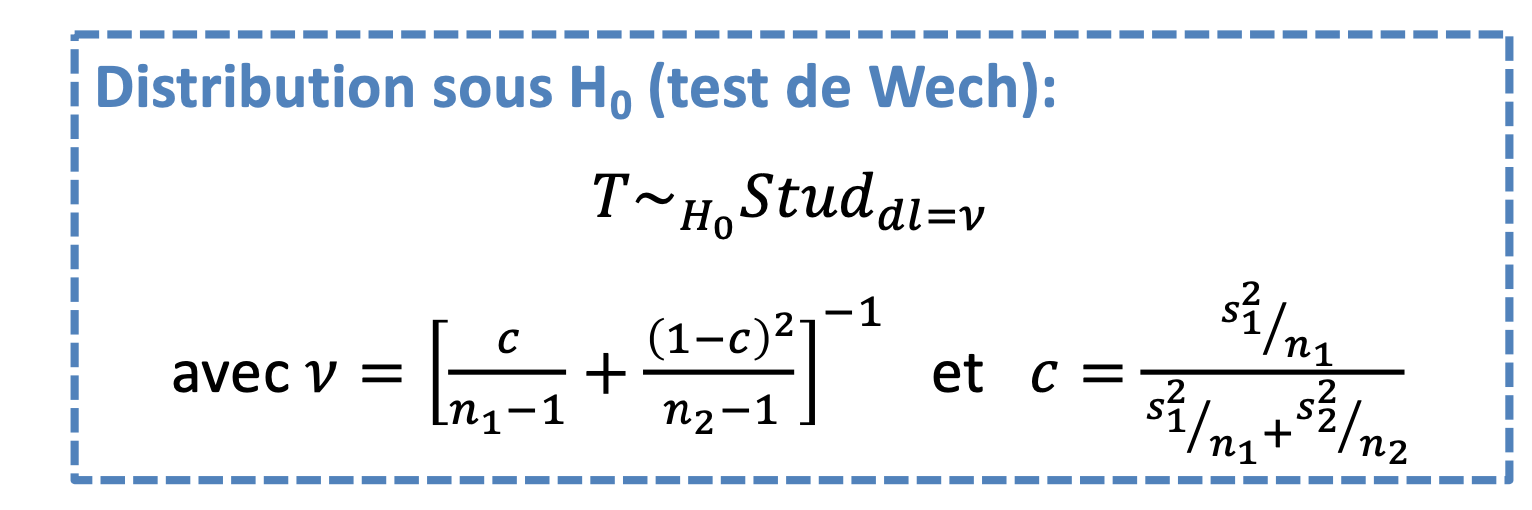
\includegraphics[scale = 0.5]{images/Welch.png}
    \caption{Test de Welch}
    \label{fig:welch}
\end{figure}

\subsubsection{Cas des données pairées}
Chaque observation du groupe 1 est liée à une (et une seule)
observation du groupe 2. On va faire un Test T pairé: pour chaque paire (i=1, ..., N) on considère la différence $d$

\begin{figure}[H]
    \centering
    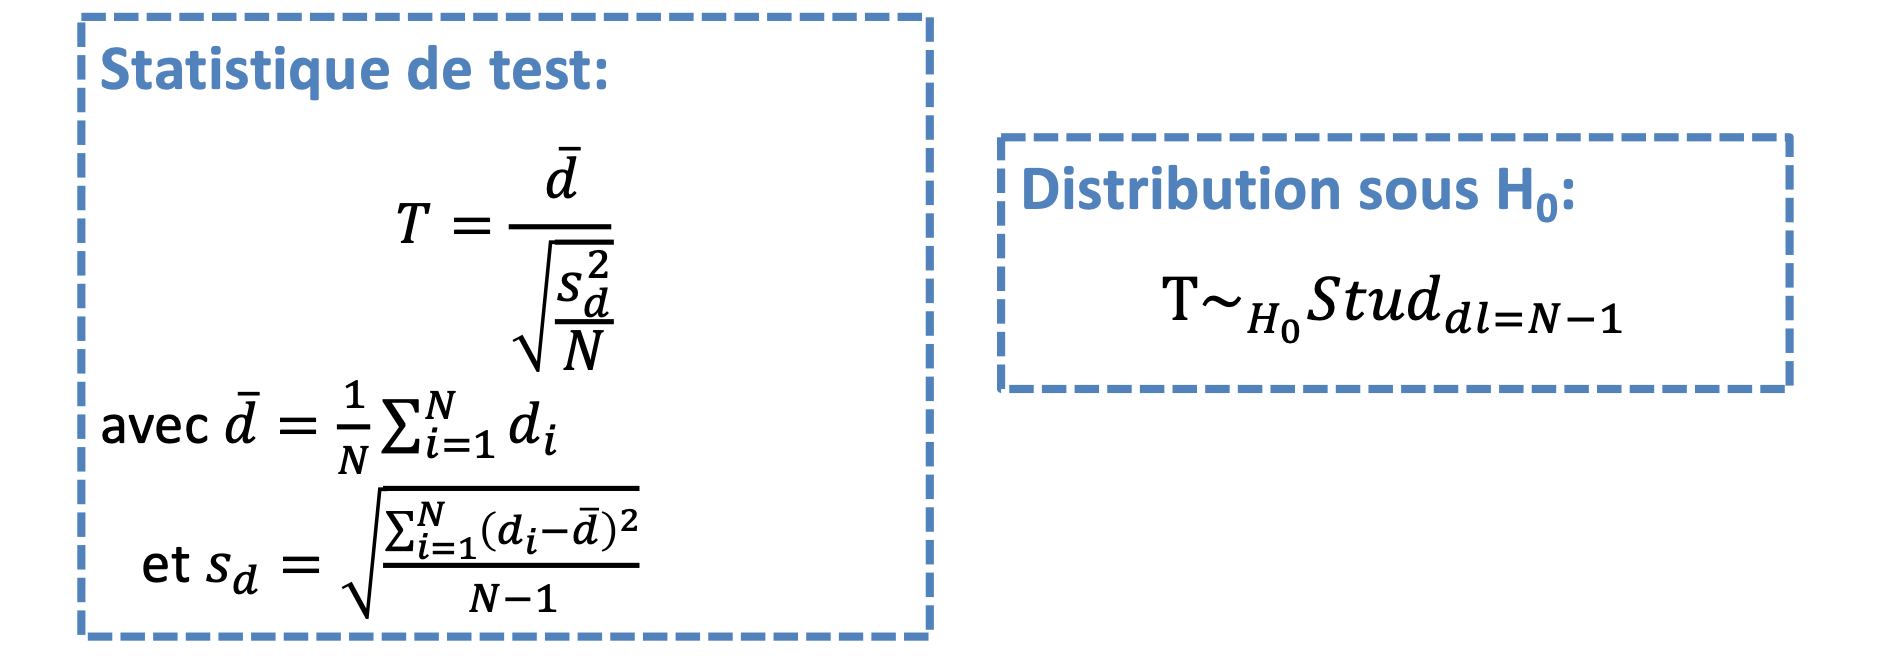
\includegraphics[scale = 0.5]{images/testTpaire.png}
    \caption{Test T pairé}
    \label{fig:my_label}
\end{figure}

\subsubsection{Estimation de l'effet traitement}
Pour un endpoint continu (approximativement normal), l’effet du traitement est typiquement résumé par l’estimation de la différence des moyennes $\mu_{1}-\mu_{2}$  et son intervalle de confiance à $1 − \alpha \%$
\subsection{Cas de plus de 2 groupes de traitement}
\textbf{Idée}: faire toutes les comparaisons deux à deux.\\ 

\textbf{MAIS}: le nombre de tests augmentent rapidement.
$$\tilde{n} = \frac{k*(k+1)}{2}$$

Il y a deux façons de définir l’erreur de type I dans le contexte de comparaisons multiples, soit Individuel (erreur de type I pour chaque test réalisé) ou Global (probabilité de faire au moins une erreur de
type I à un des tests [Family error rate])

Le risque global d’erreur de type I augmente (très rapidement) avec le nombre de comparaisons\\

$$\alpha_{G}=1-(1-\alpha)^{n_{k}}$$

\begin{figure}[H]
    \centering
    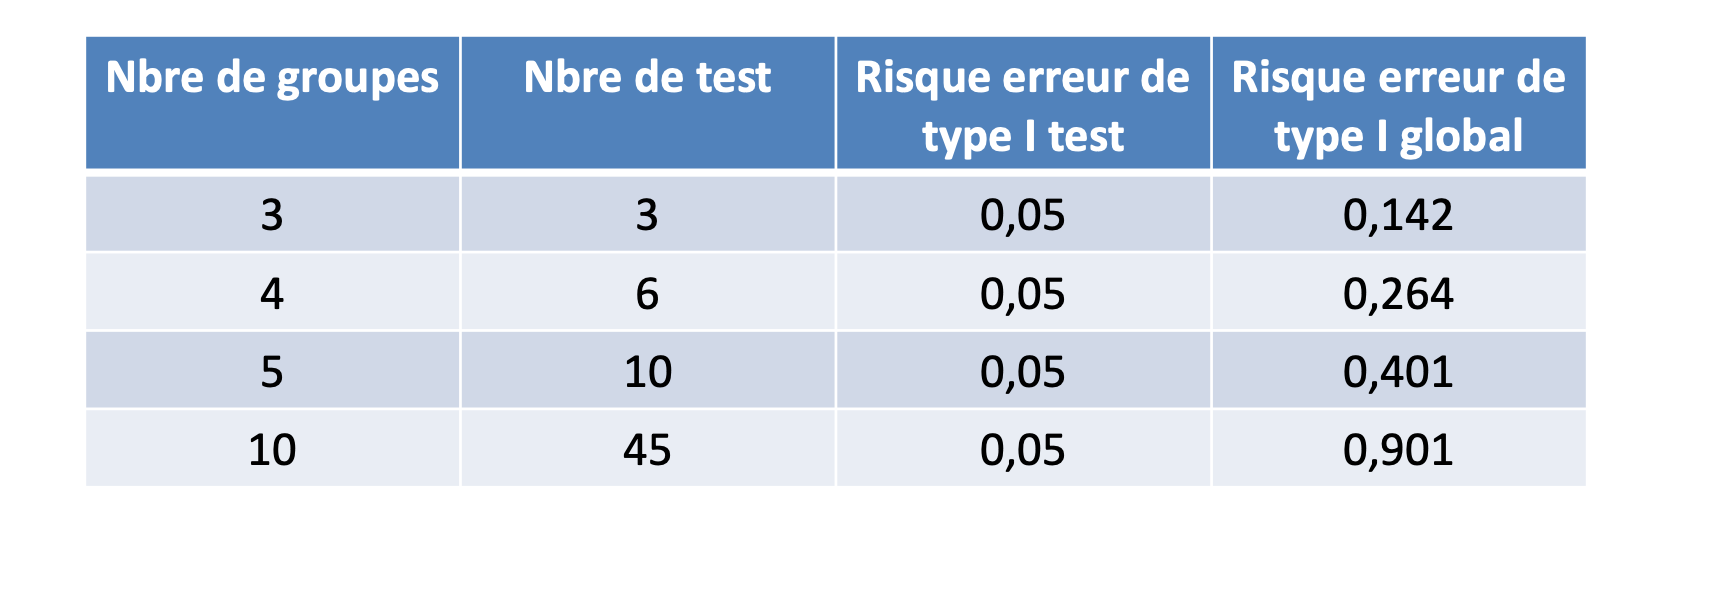
\includegraphics[scale = 0.5]{images/erreurglobal.png}
    \caption{augmentation erreur globale de type I}
    \label{fig:my_label}
\end{figure}

\begin{center}
    Donc on a des problèmes de multiplicité des tests
\end{center}

\textbf{Solutions}

\begin{figure}[H]
    \centering
    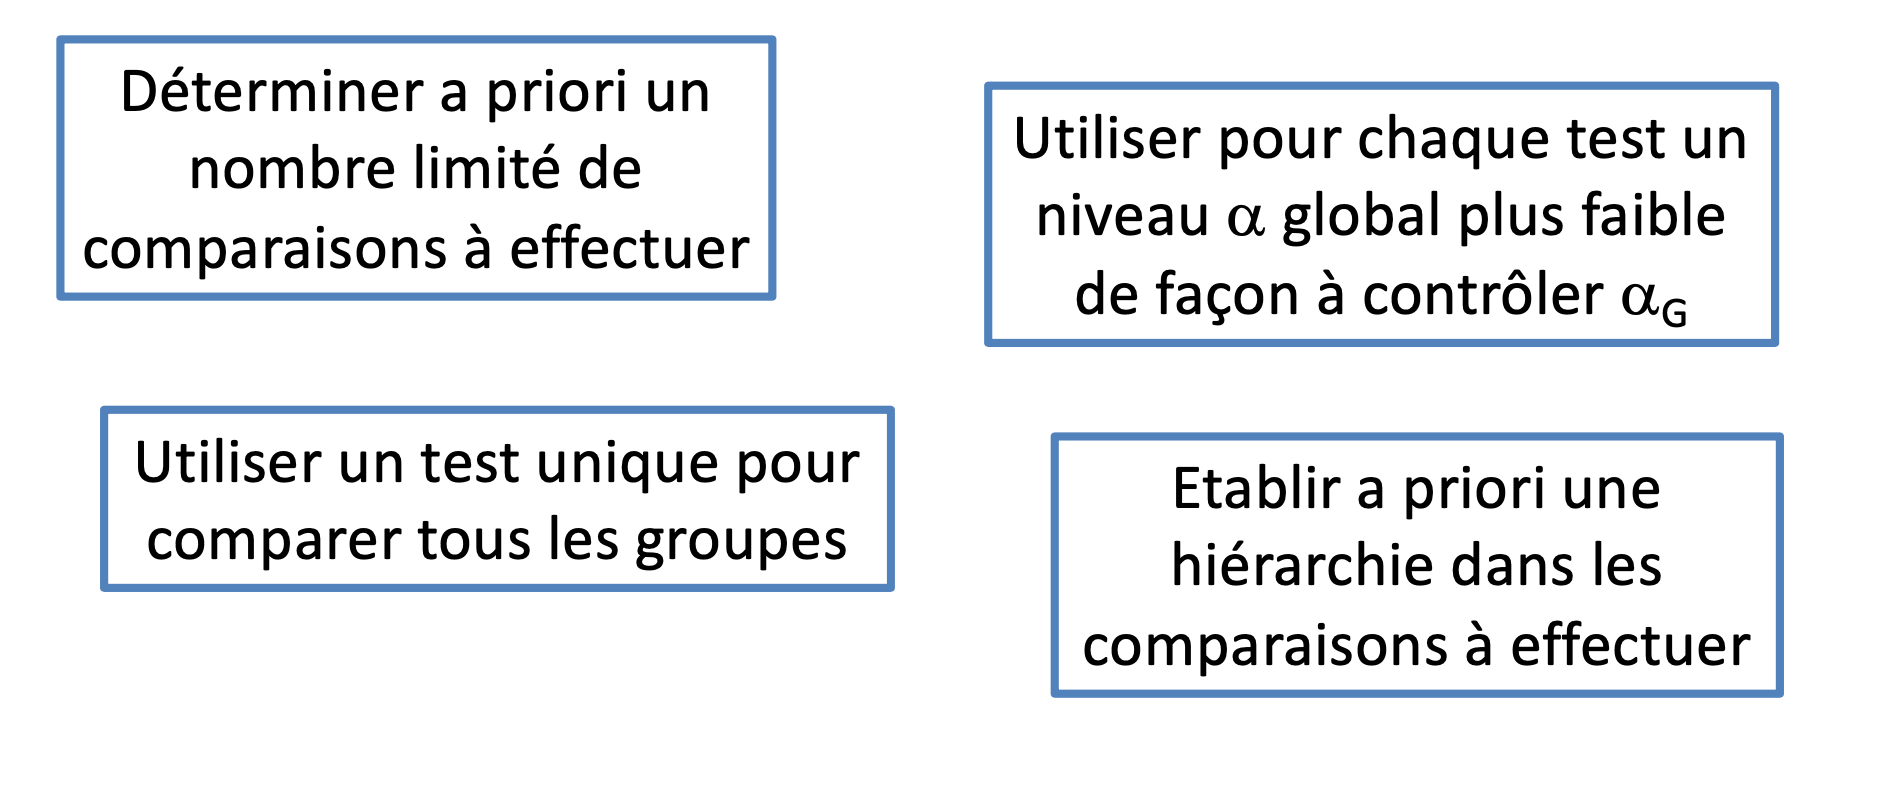
\includegraphics[scale = 0.5]{images/problememultitest.png}
    \caption{Solutions}
    \label{fig:my_label}
\end{figure}

\subsubsection{Utiliser pour chaque test un niveau a global plus faible de façon à contrôler $\alpha_{G}$:procédure de Bonferroni}
$$\tilde{\alpha}= \frac{\alpha}{\tilde{n_{k}}} \Rightarrow \alpha_{G}=1-(1-\tilde{\alpha})^{n_{k}} < \alpha$$

\subsubsection{Utiliser un test unique pour comparer tous les groupes :ANOVA}
\begin{figure}[H]
    \centering
    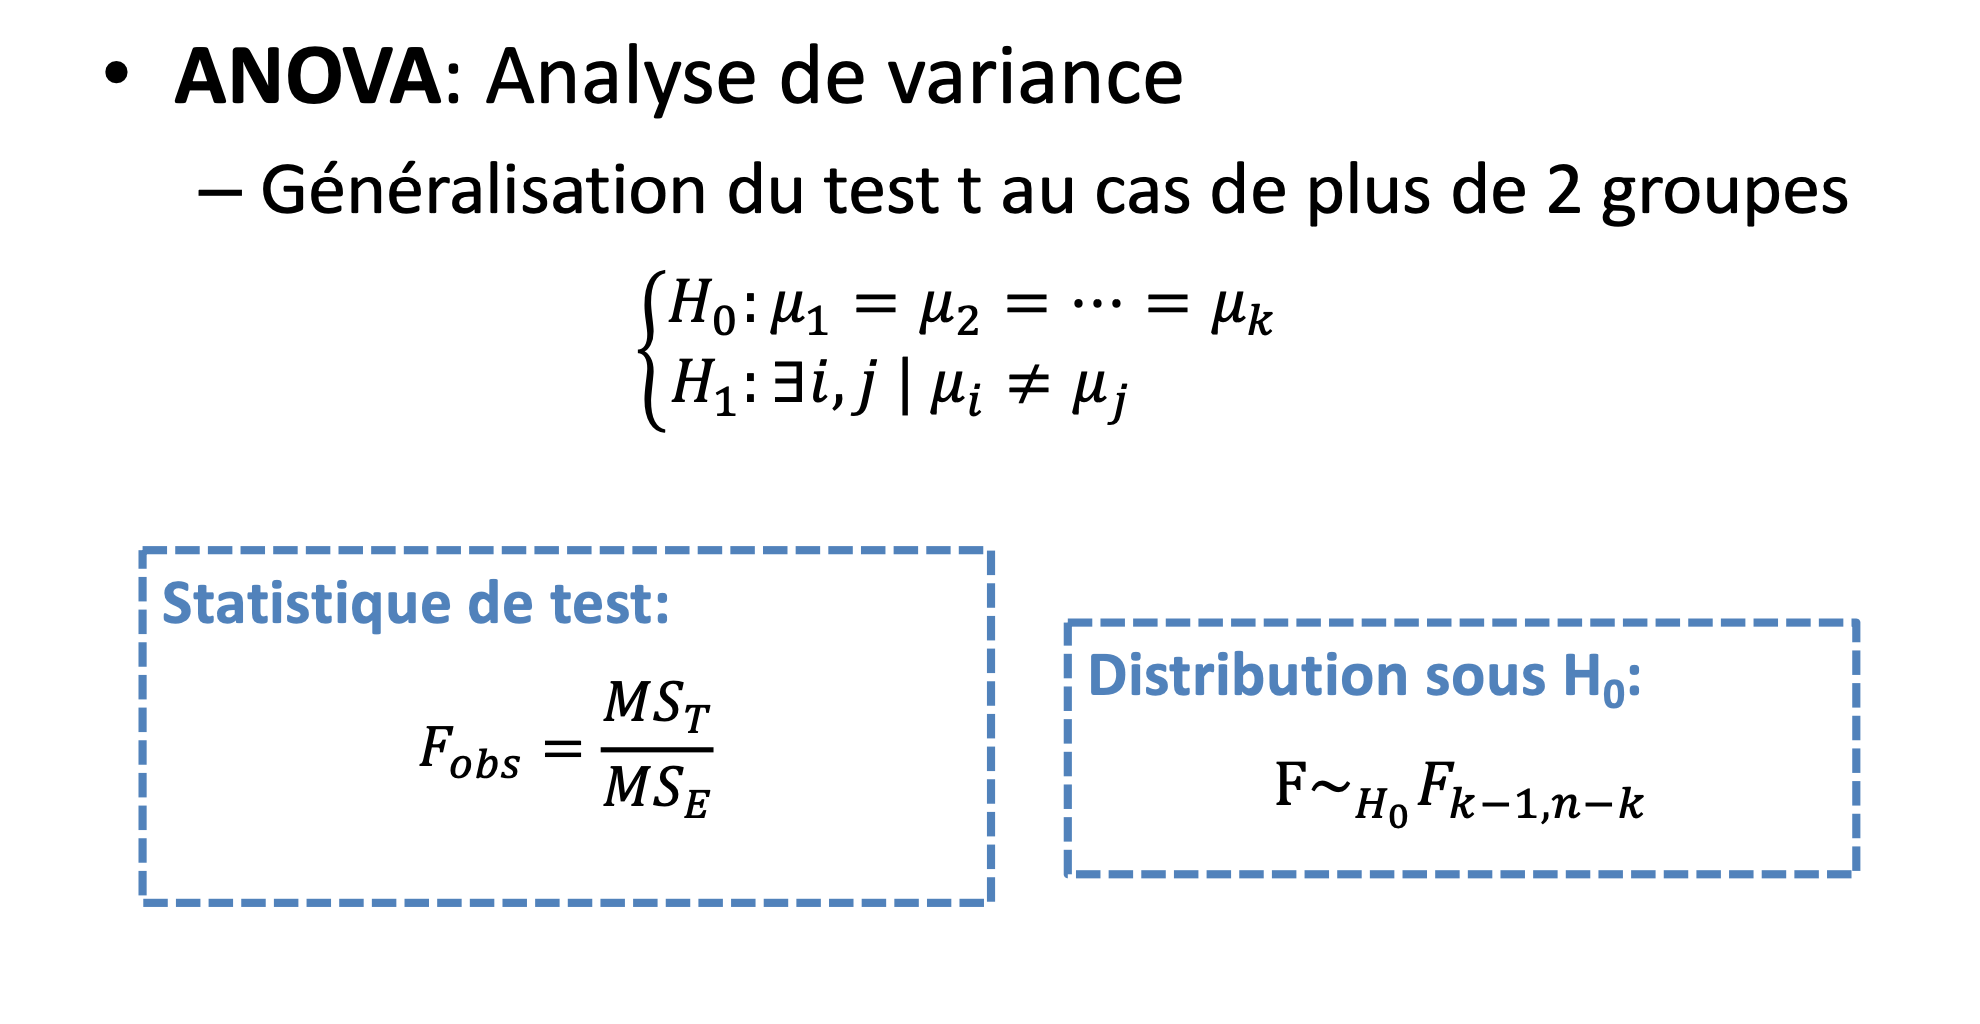
\includegraphics[scale=0.5]{images/anova.png}
    \caption{Test Anova}
    \label{fig:anova}
\end{figure}

\textbf{Remarques}
\begin{enumerate}
    \item Conditions d’applications du test F d’ANOVA:
    \begin{itemize}
        \item X est une variable continue de distribution (approximativement) normale, et de même variance dans toutes les sous-populations considérées
        \item Les observations sont indépendants
    \end{itemize}
    \item On présente souvent les résultats sous la forme d’une table d’ANOVA
    \item Si RHO, il faut encore déterminer quels sont les groupes qui ont des moyennes différentes ! Il faut alors calculer les intervalles de confiance pour les différences de moyennes deux à deux.
\end{enumerate}

Pour résoudre le problème de multiplicité, on plusieurs possibilités :
\begin{itemize}
    \item Méthode LSD de Fisher
    \item Méthode de Tukey-Kramer
    \item Méthode de Dunnett
    \item ...
\end{itemize}

\begin{figure}[H]
    \centering
    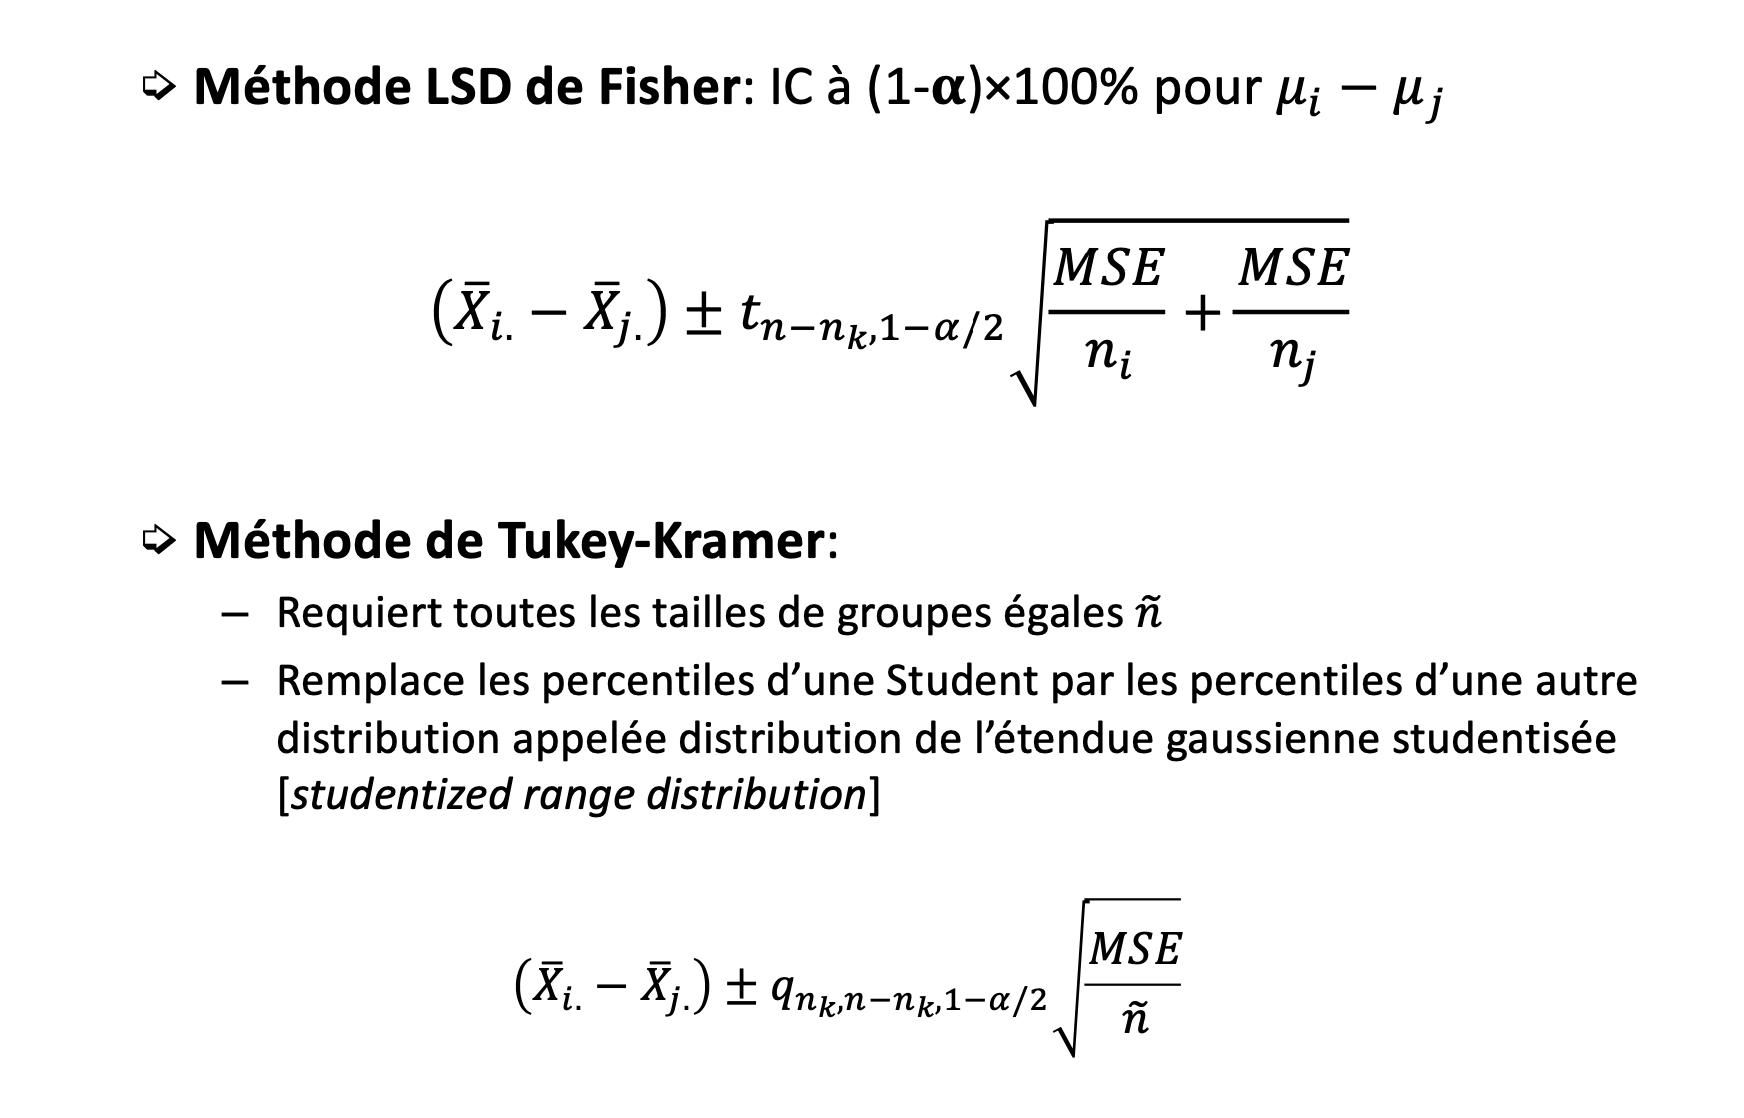
\includegraphics[scale=0.4]{images/LSD_Tukey.png}
    \caption{Méthode de LSD de Fisher et de Tukey-Kramer}
    \label{fig:my_label}
\end{figure}

\begin{figure}[H]
    \centering
    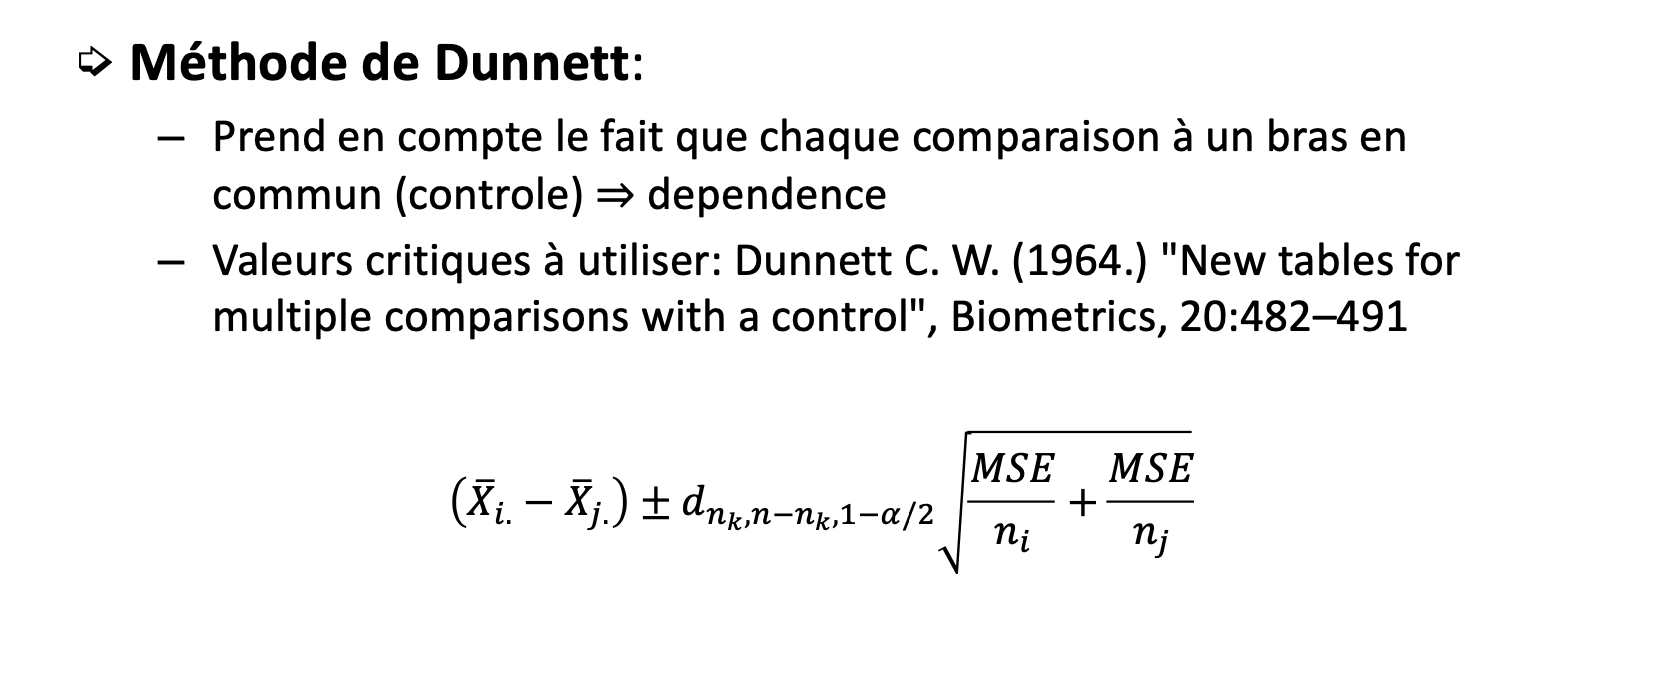
\includegraphics[scale=0.4]{images/Dunnett.png}
    \caption{Méthode de LSD de Dunnett}
    \label{fig:my_label}
\end{figure}


\subsection{Régression linéaire multiple}
On décrit l’association (linéaire) entre Une variable Y (= réponse) continue et plusieurs variables X explicatives.

\begin{figure}[H]
    \centering
    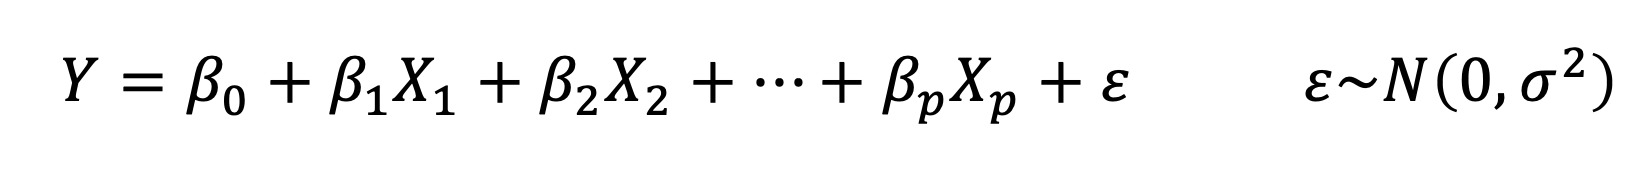
\includegraphics[scale = 0.5]{images/regressionlineaire.png}
    \caption{formule régression linéaire}
    \label{fig:my_label}
\end{figure}
On trouve les valeurs de  soit par le critère des moindres carrées soit par la méthode du maximum de vraisemblance.\\

On peut interpréter $\beta_k$ comme le changement moyen de la valeur de Y quand $X_{k}$ augmente d’une unité (les valeurs de toutes les autres variables étant fixée).

\section{Endpoint binaire}
Pour chaque patient, l’endpoint binaire se mesure comme étant : Succès ou Échec. 

\subsection{Cas de deux groupes de traitements}

\begin{figure}[H]
    \centering
    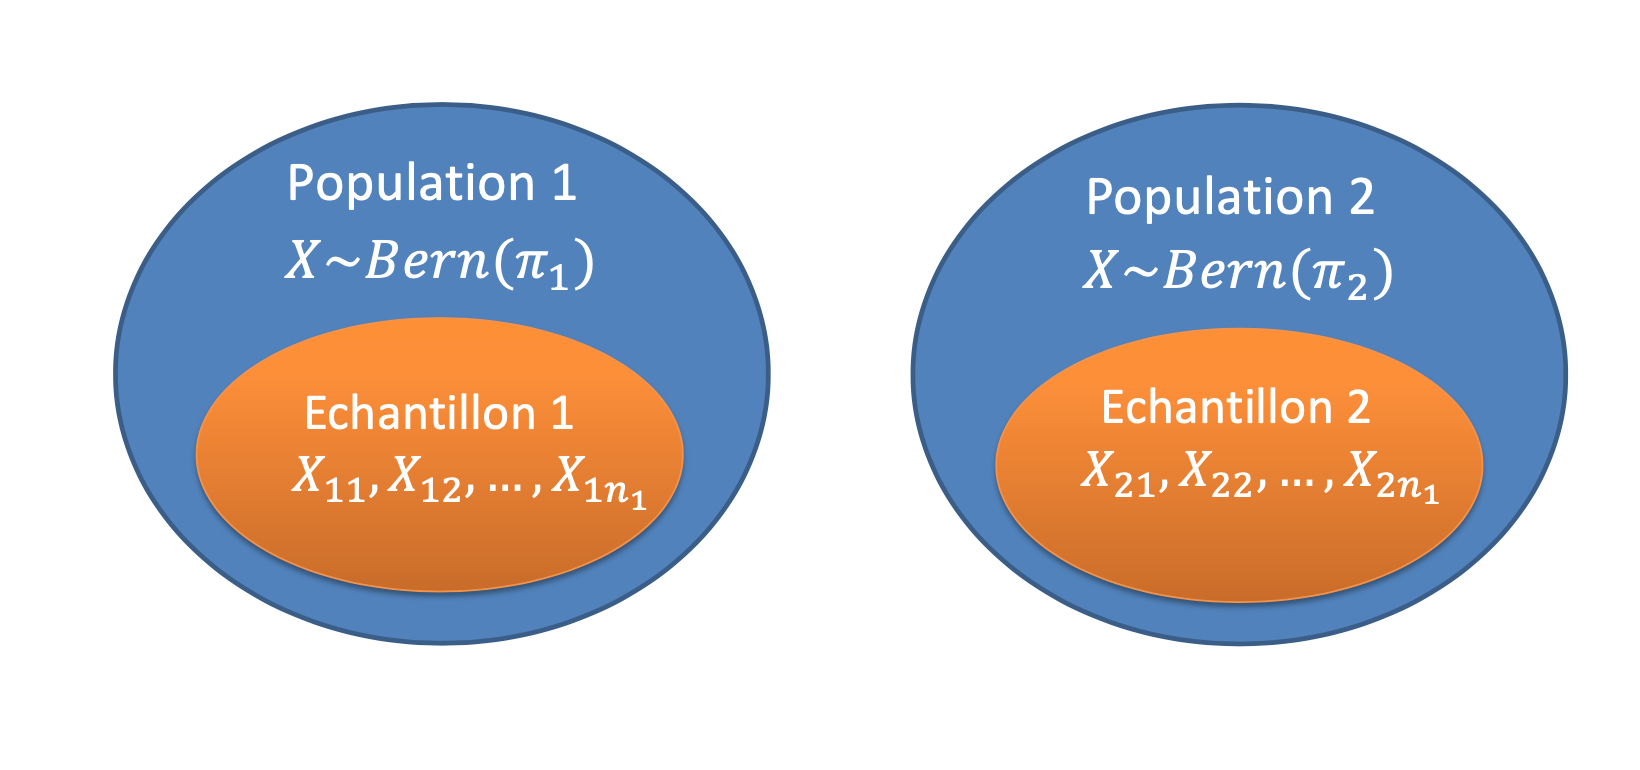
\includegraphics[scale = 0.5]{images/deuxgroupesbinaires.png}
    \caption{Cas de deux groupes de traitements}
    \label{fig:my_label}
\end{figure}

\subsubsection{Test Z pour comparer deux probabilités}

\begin{figure}[H]
    \centering
    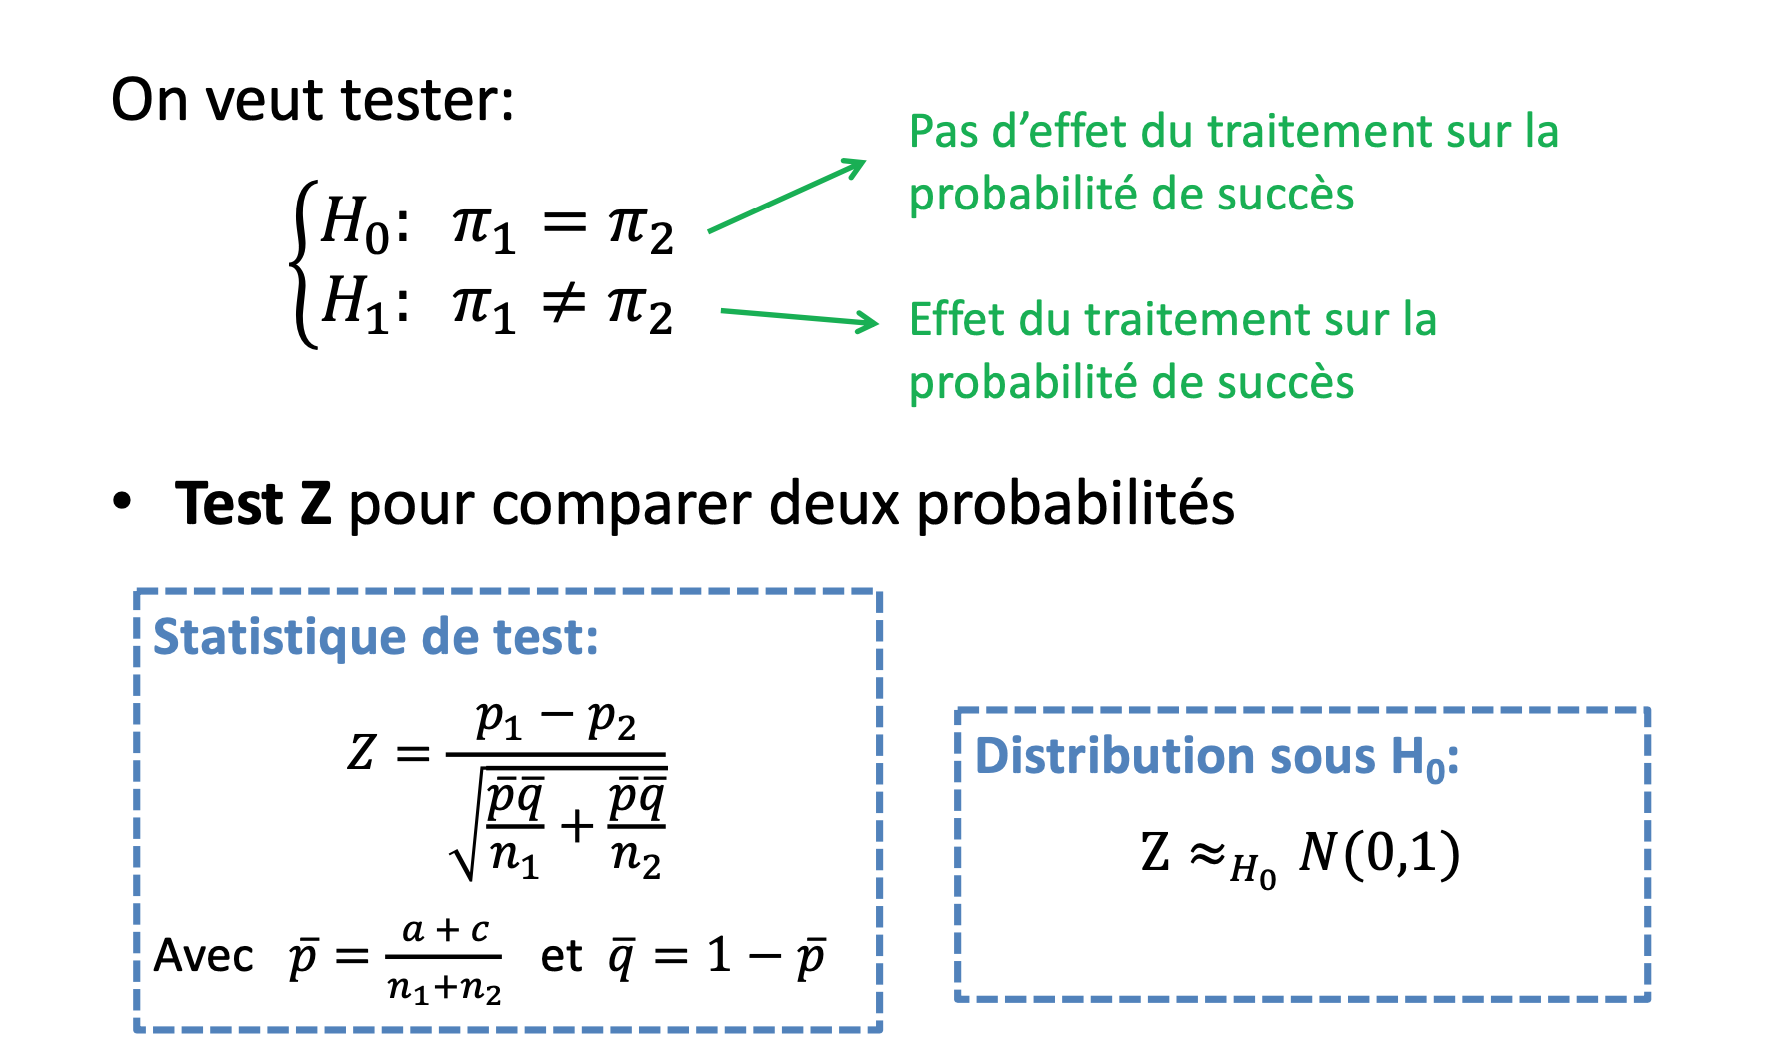
\includegraphics[scale=0.5]{images/testZ.png}
    \caption{Test Z pour comparer deux probabilités}
    \label{fig:my_label}
\end{figure}


\subsubsection{Test Chi-carré d’indépendance} 
\begin{figure}[H]
    \centering
    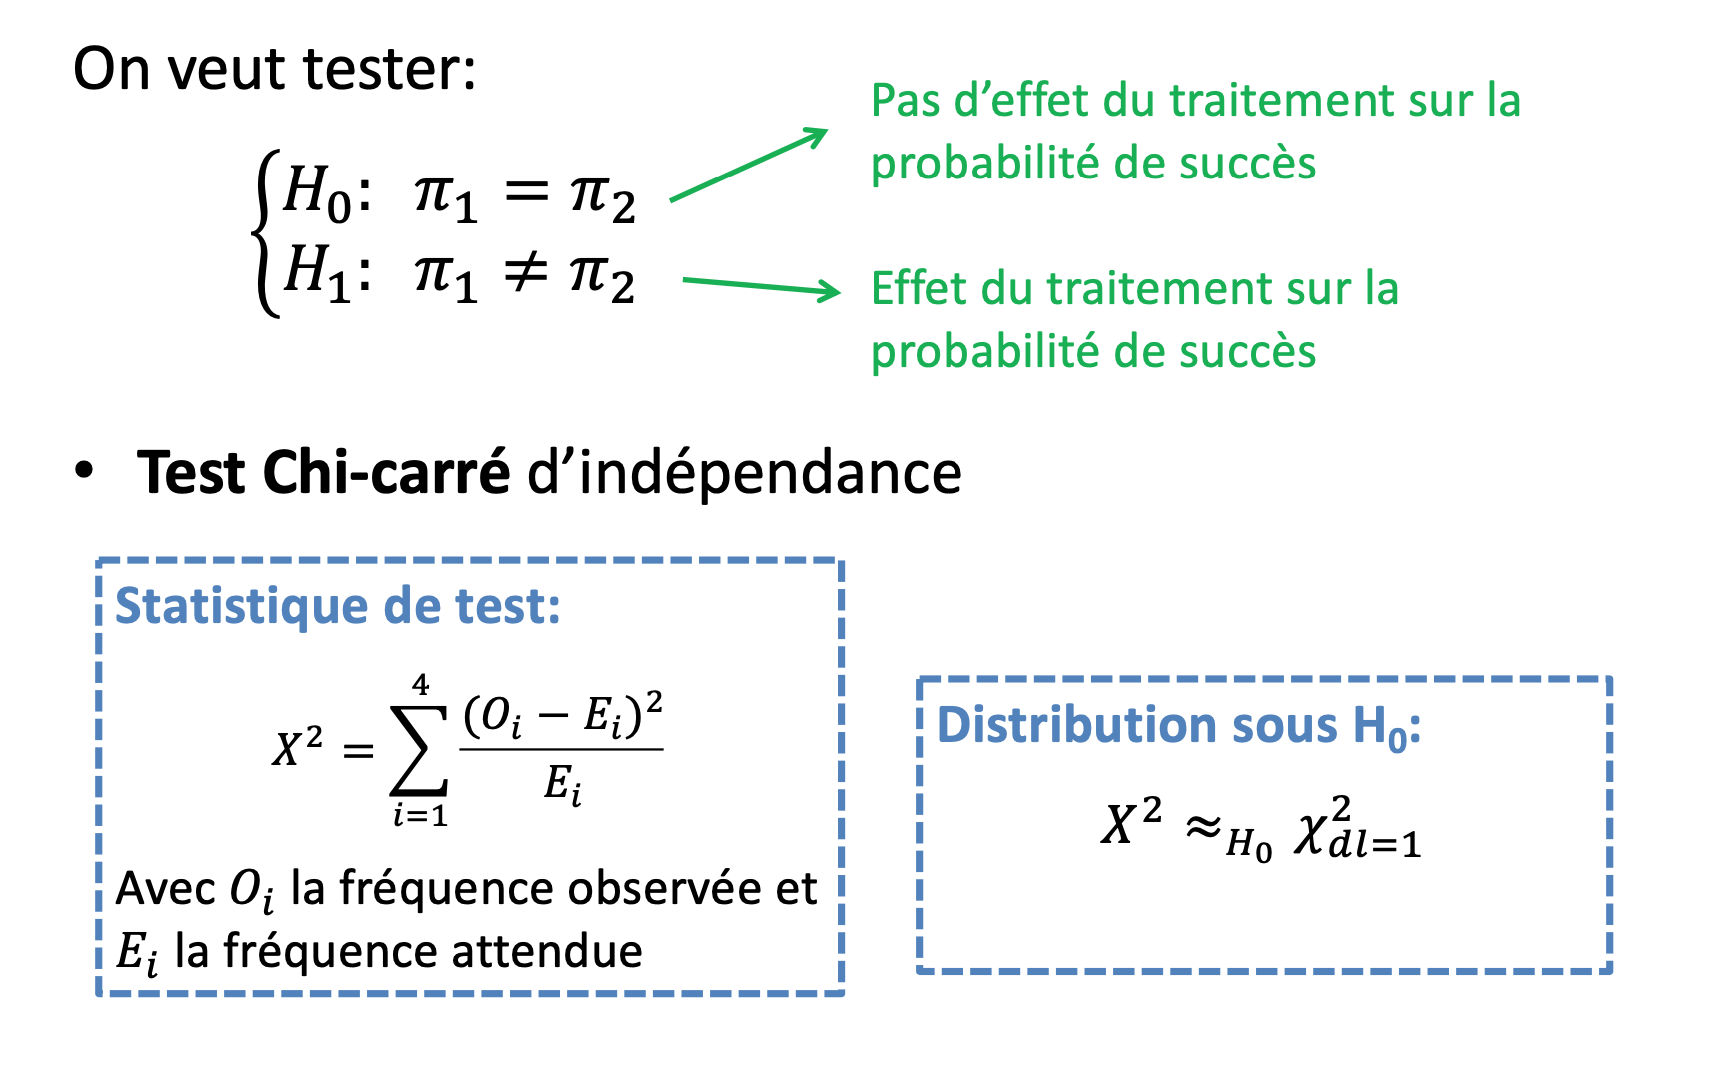
\includegraphics[scale =0.5]{images/testchisquare.png}
    \caption{Test Chi carré d'indépendance}
    \label{fig:my_label}
\end{figure}

\subsubsection{Remarques}
\begin{enumerate}
    \item Le test chi-carré est en fait équivalent au test Z, basé sur l’approximation normale de la distribution binomiale.
    $$X^{2} = (Z)^{2}$$
    \item Il existe aussi un test chi-carré avec une correction de continuité
    \begin{itemize}
        \item La statistique de test classique ne peut en réalité prendre qu’un nombre discret de valeurs alors que la distribution théorique (chi-carré) est une distribution continue.
        \item Le calcul de la P-valeur est approximatif, et on ne peut donc ne pas exactement contrôler $\alpha$ (surtout lorsque dl=1).
        \item Il est alors recommandé d’utiliser la correction de continuité de Yates (Yates,1934) Figure \ref{fig:Yates}.
    \end{itemize}
    \item Ces résultats reposent sur le TCL et sont asymptotiques.
    \begin{itemize}
        \item Si taille d’échantillon petite, mais toutes les fréquences attendues >5 : test chi-carré OK avec correction de continuité de Yates
        \item Si au moins une fréquence attendue $\leqslant 5$, alors le test chi-carré et le test Z ne peuvent pas être utilisé. On peut alors réaliser un test exact de Fischer
    \end{itemize}
\end{enumerate}

\begin{figure}[H]
    \centering
    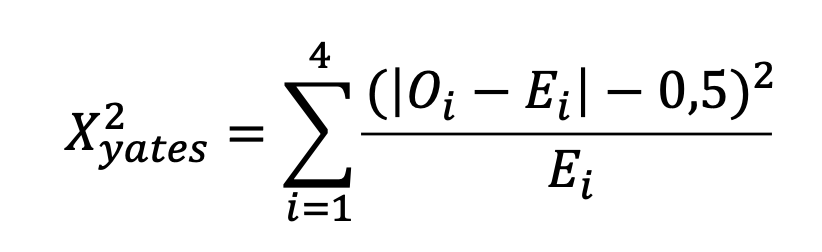
\includegraphics[scale = 0.5]{images/Yates.png}
    \caption{Correction de continuité de Yates}
    \label{fig:Yates}
\end{figure}

\subsubsection{Cas des données pairées}

\begin{figure}[H]
    \centering
    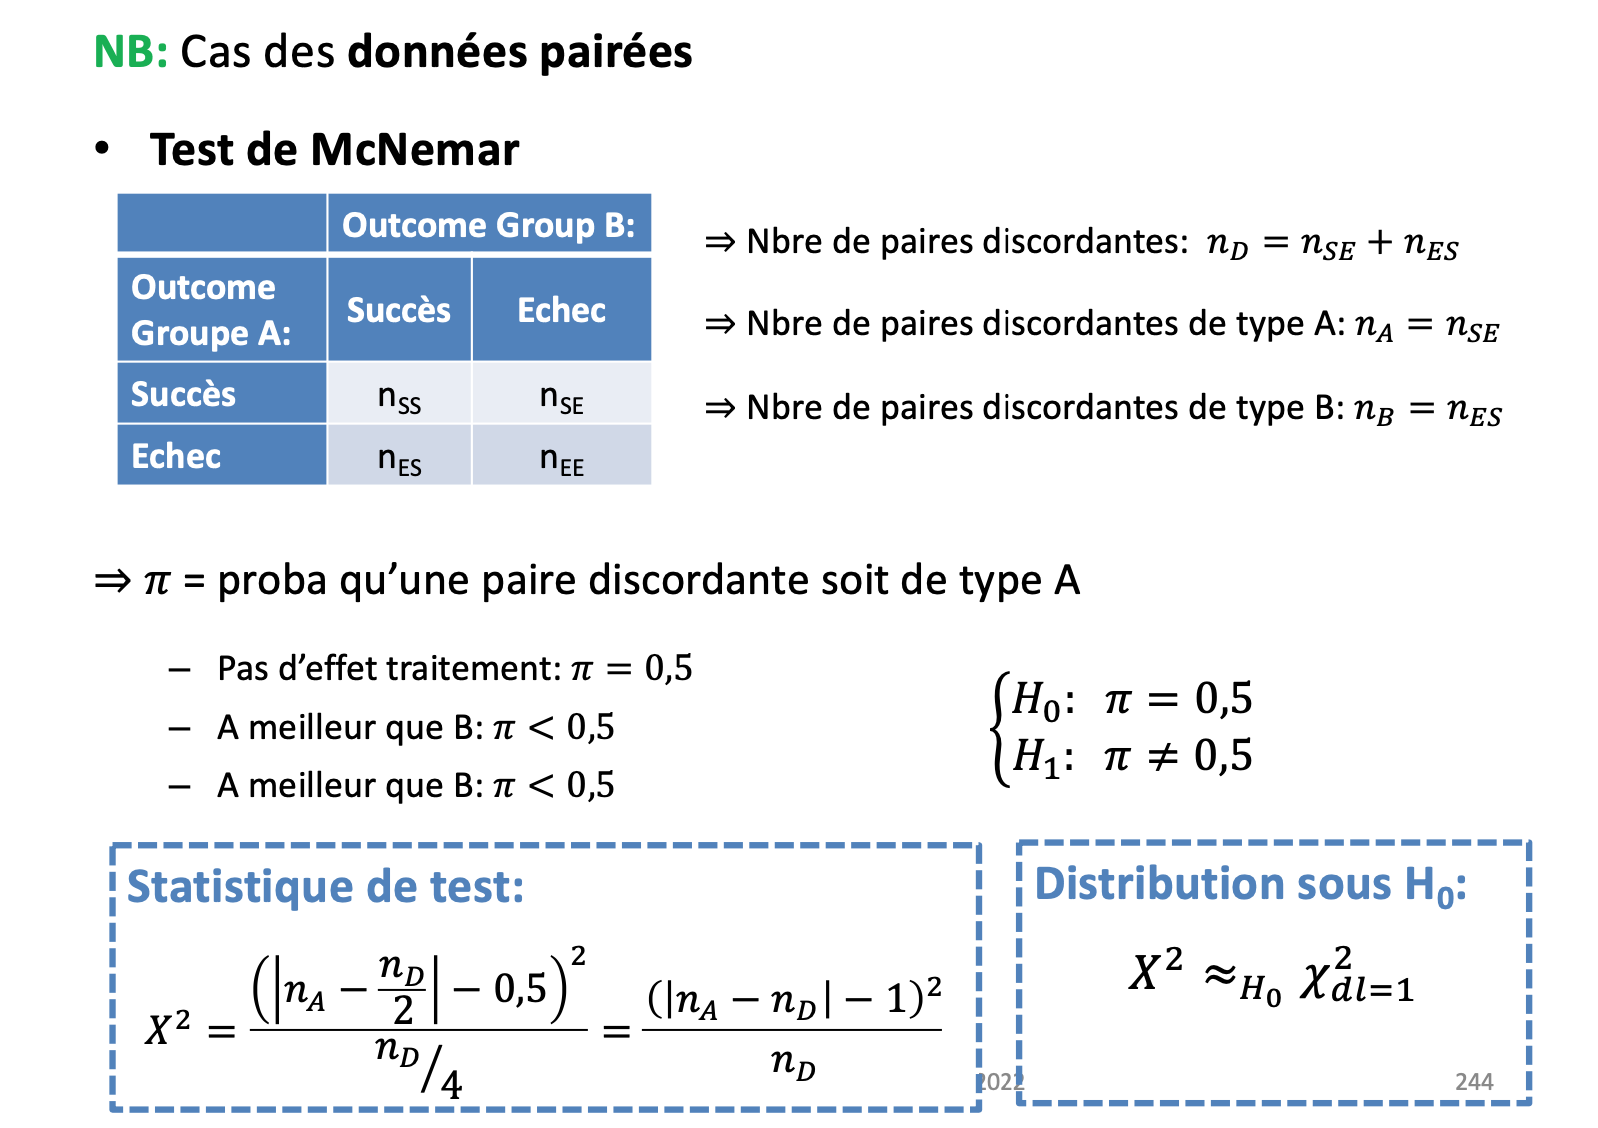
\includegraphics[scale = 0.5]{images/donnespaires.png}
    \caption{Test statistique dans le cas de données pairées}
    \label{fig:paires}
\end{figure}

\subsection{Estimation effet traitement}

Différentes possibilités :
\begin{itemize}
    \item Différence des proportions estimées
    \item Rapport de risques (Risks ratio, RR) estimé
    \item Rapport de cotes (Odds ratio, OR) estimé
\end{itemize}

\subsubsection{Différence des proportions estimées}
Cette technique consiste à faire la différence entre les deux probabilités de succès. Mais c'est rarement utilisé !

\subsubsection{Rapport de risques (Risks ratio, RR) estimé}
Cette technique revient à faire le ratio des proportions estimées. Le RR peut se calculer dans les études prospectives (et donc dans les essais cliniques) mais pas dans les études rétrospectives de type cas-contrôle.
$$\hat{RR} = \frac{\hat{\pi_{1}}}{\hat{\pi_{2}}}=\frac{p_{1}}{p_{2}} $$
Pour l'interprétation :
\begin{figure}[H]
    \centering
    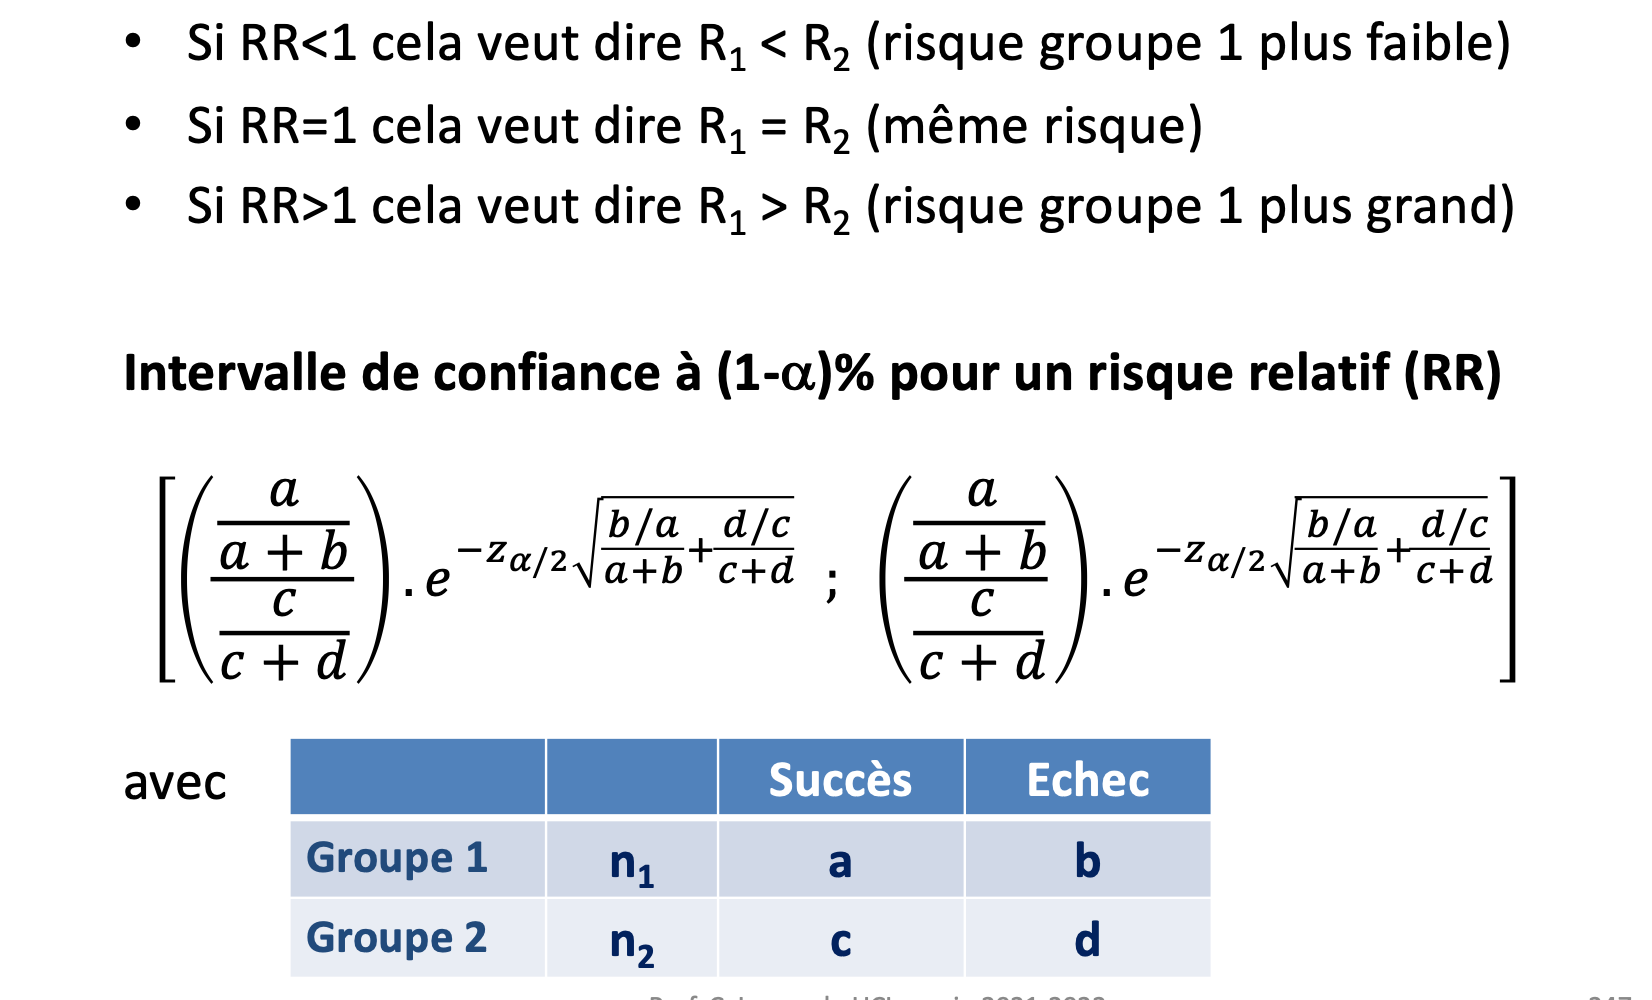
\includegraphics[scale = 0.5]{images/interpretationrisqueration.png}
    \caption{Interprétation du rapport de risque}
    \label{fig:my_label}
\end{figure}

\subsubsection{Rapport de cotes (Odds ratio, OR) estimé}

Cote = probabilité de succès sur probabilité d’échec.

\begin{figure}[H]
    \centering
    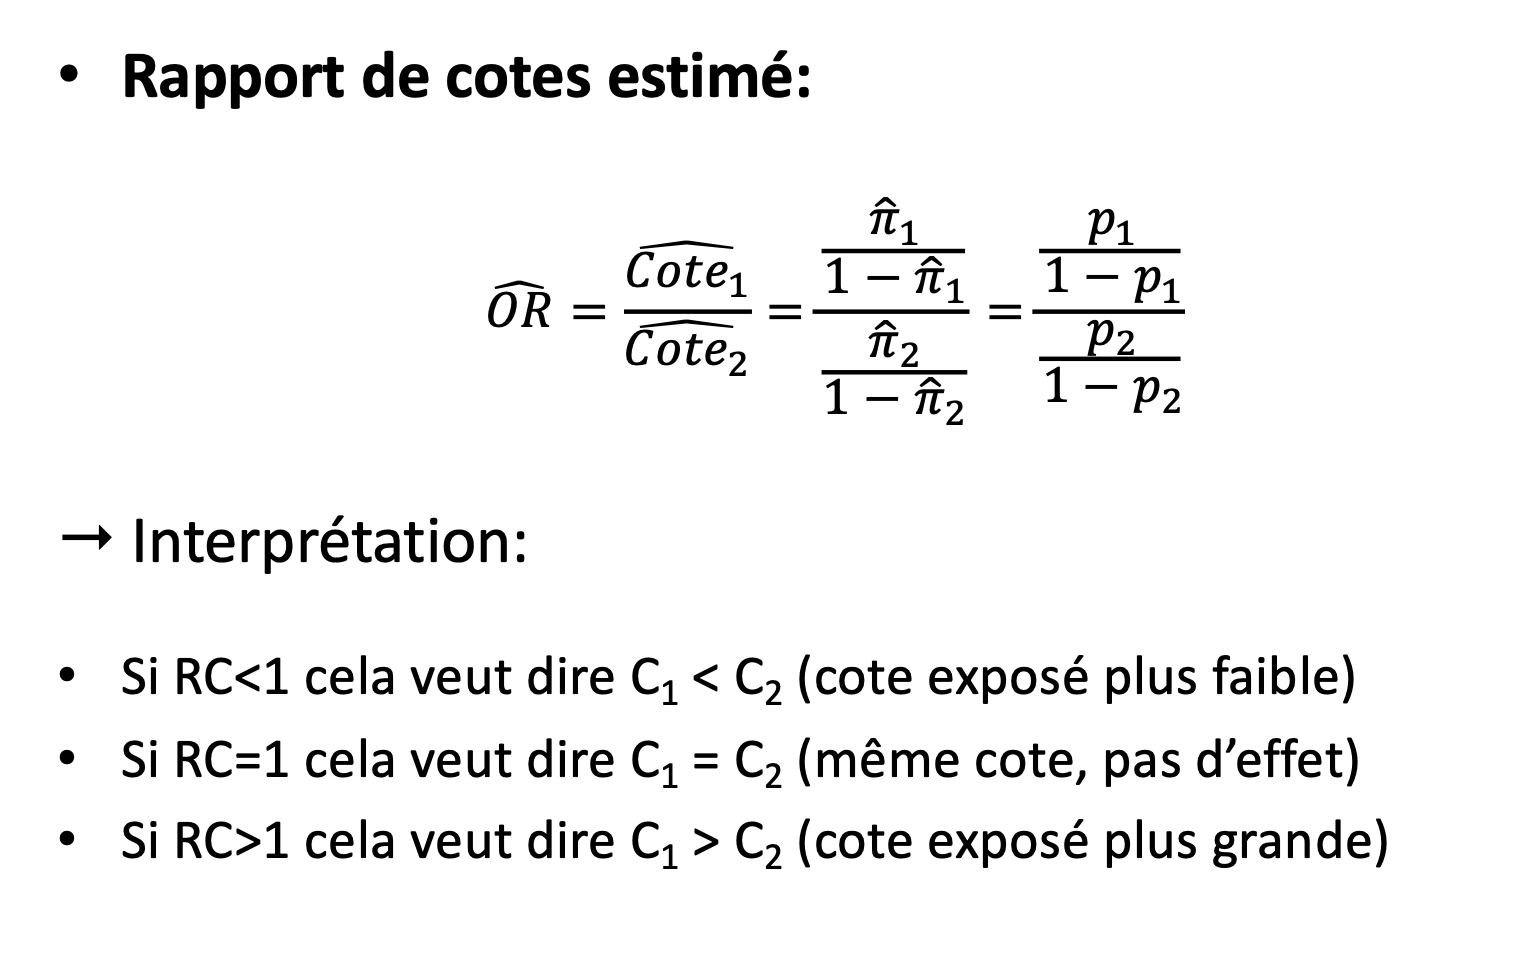
\includegraphics[scale=0.5]{images/rapportdescotes.png}
    \caption{Interprétation rapport des côtes}
    \label{fig:my_label}
\end{figure}


\begin{figure}[H]
    \centering
    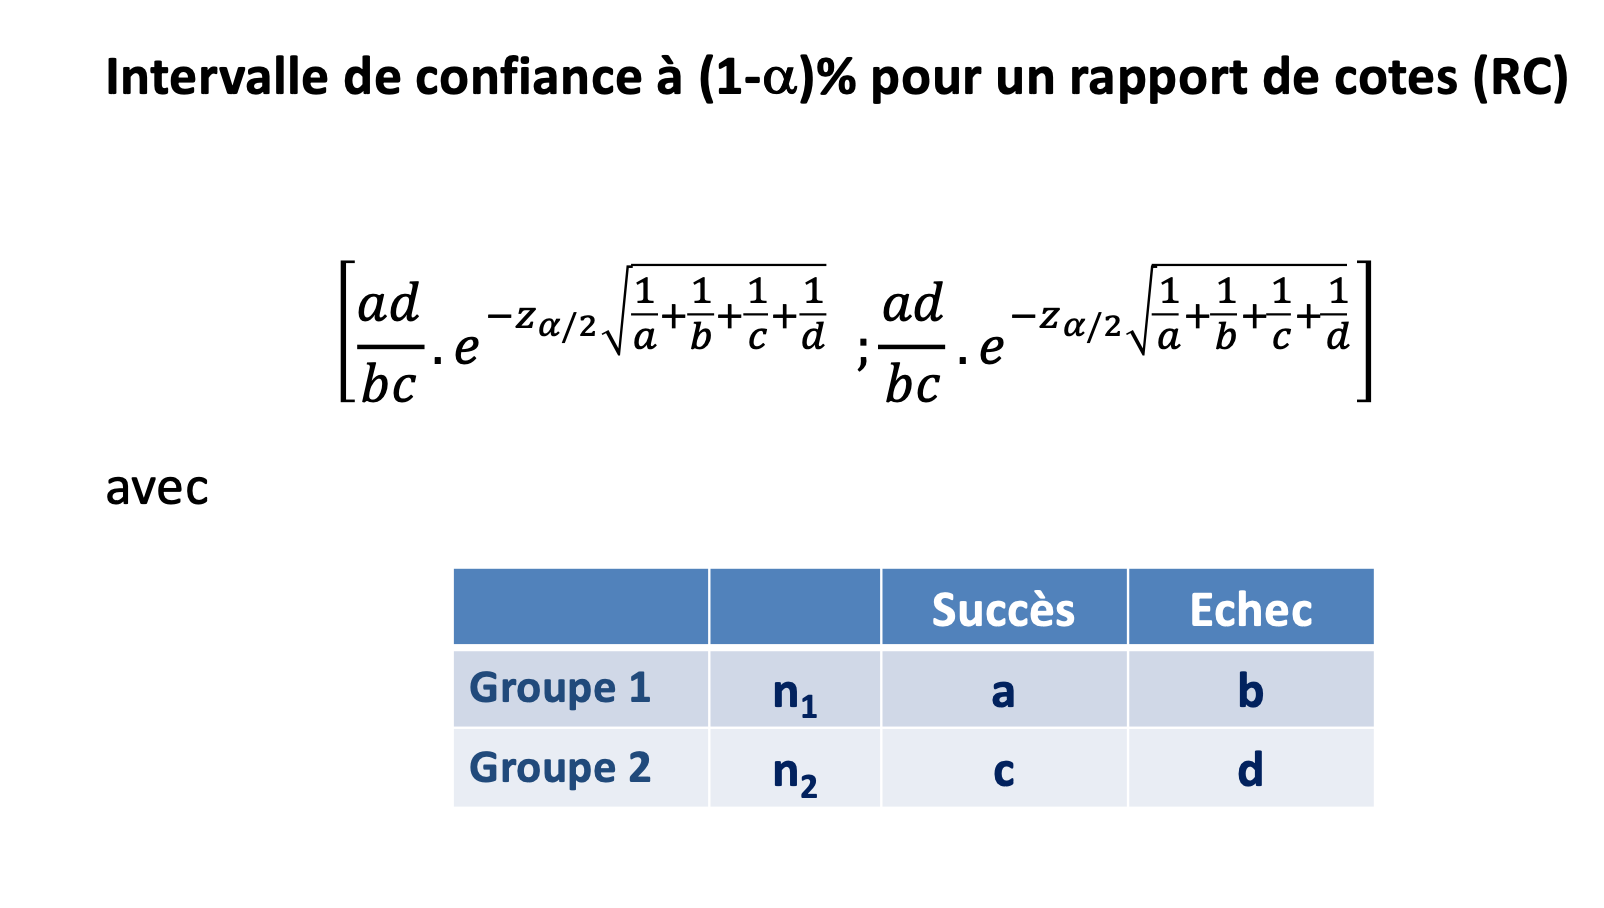
\includegraphics[scale=0.5]{images/intervaldeconfiance.png}
    \caption{Intervalle de confiance du rapport des côtes}
    \label{fig:my_label}
\end{figure}
Il faut attention à la manière d'interpréter le RR et OR. Ils ont la même interprétation qualitative, mais pas quantitative.
\begin{figure}[H]
    \centering
    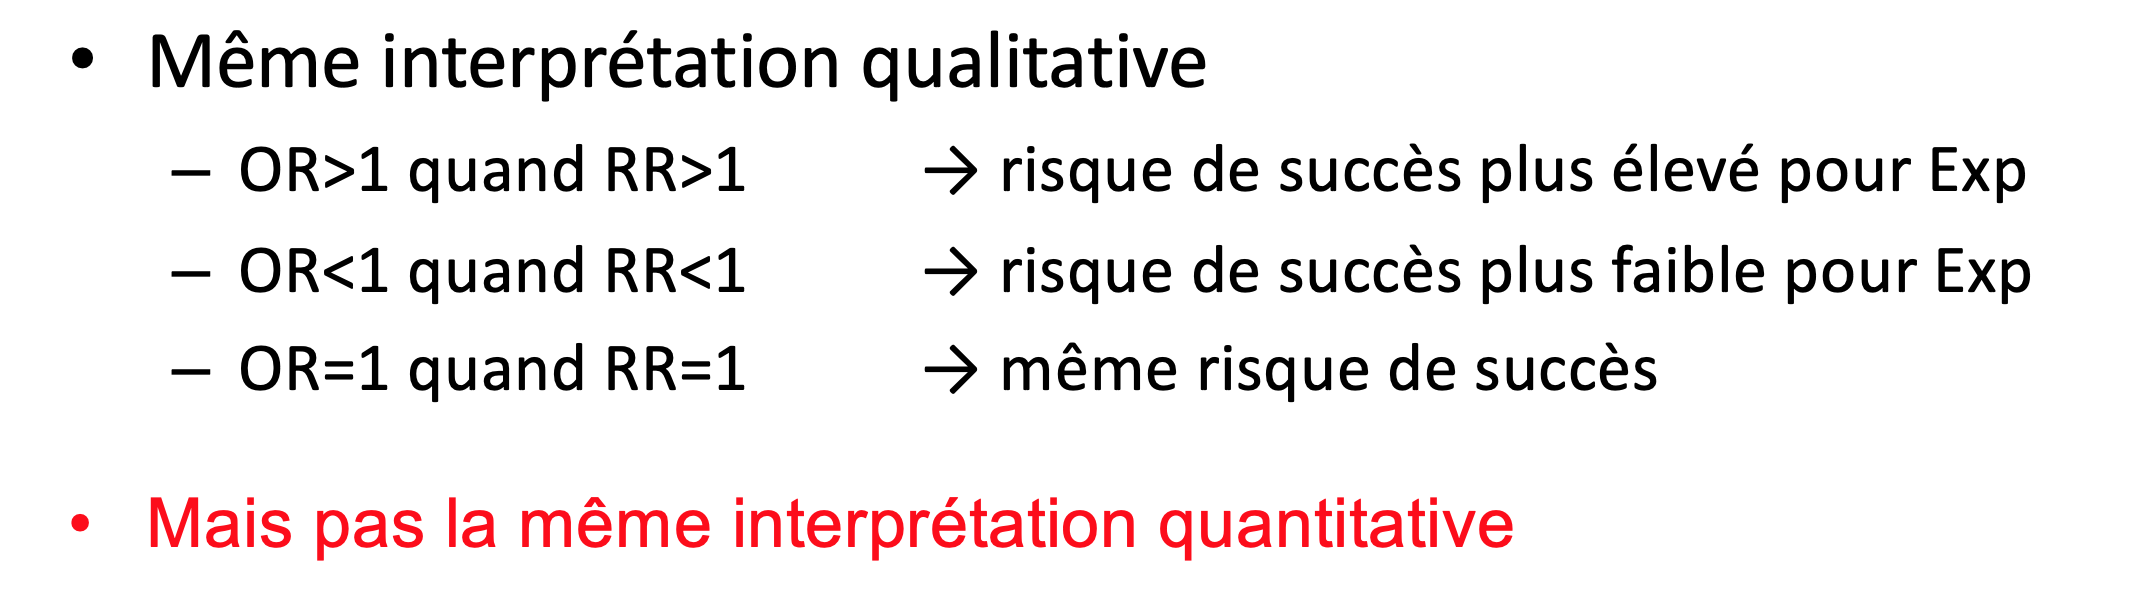
\includegraphics[scale =0.3]{images/RROR.png}
    \caption{Interprétation RR et OR}
    \label{fig:RROR}
\end{figure}
\subsection{Régression logistique}
On ne peut pas faire une régression linéaire, car nous avons une variable de réponse binaire Y (= 0 pour échec ou 1 pour succès) et un ou plusieurs facteurs : $X=(X_{1}, ..., X_{k})$\\

On voudrait modéliser le risque $\pi = P(Y=1|X)$. Mais En réalité, on va modéliser le logarithme de la cote, c.-à-d. le logit de $\pi$.

\begin{figure}[H]
    \centering
    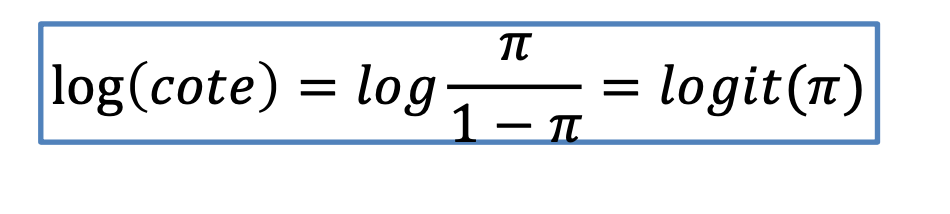
\includegraphics[scale = 0.3]{images/logit.png}
    \caption{Formule logit}
    \label{fig:my_label}
\end{figure}

$$ logit(\pi) = \beta_{0}+\beta_{1}X_{1}+...+\beta_{n}X_{n}$$

\begin{figure}[H]
    \centering
    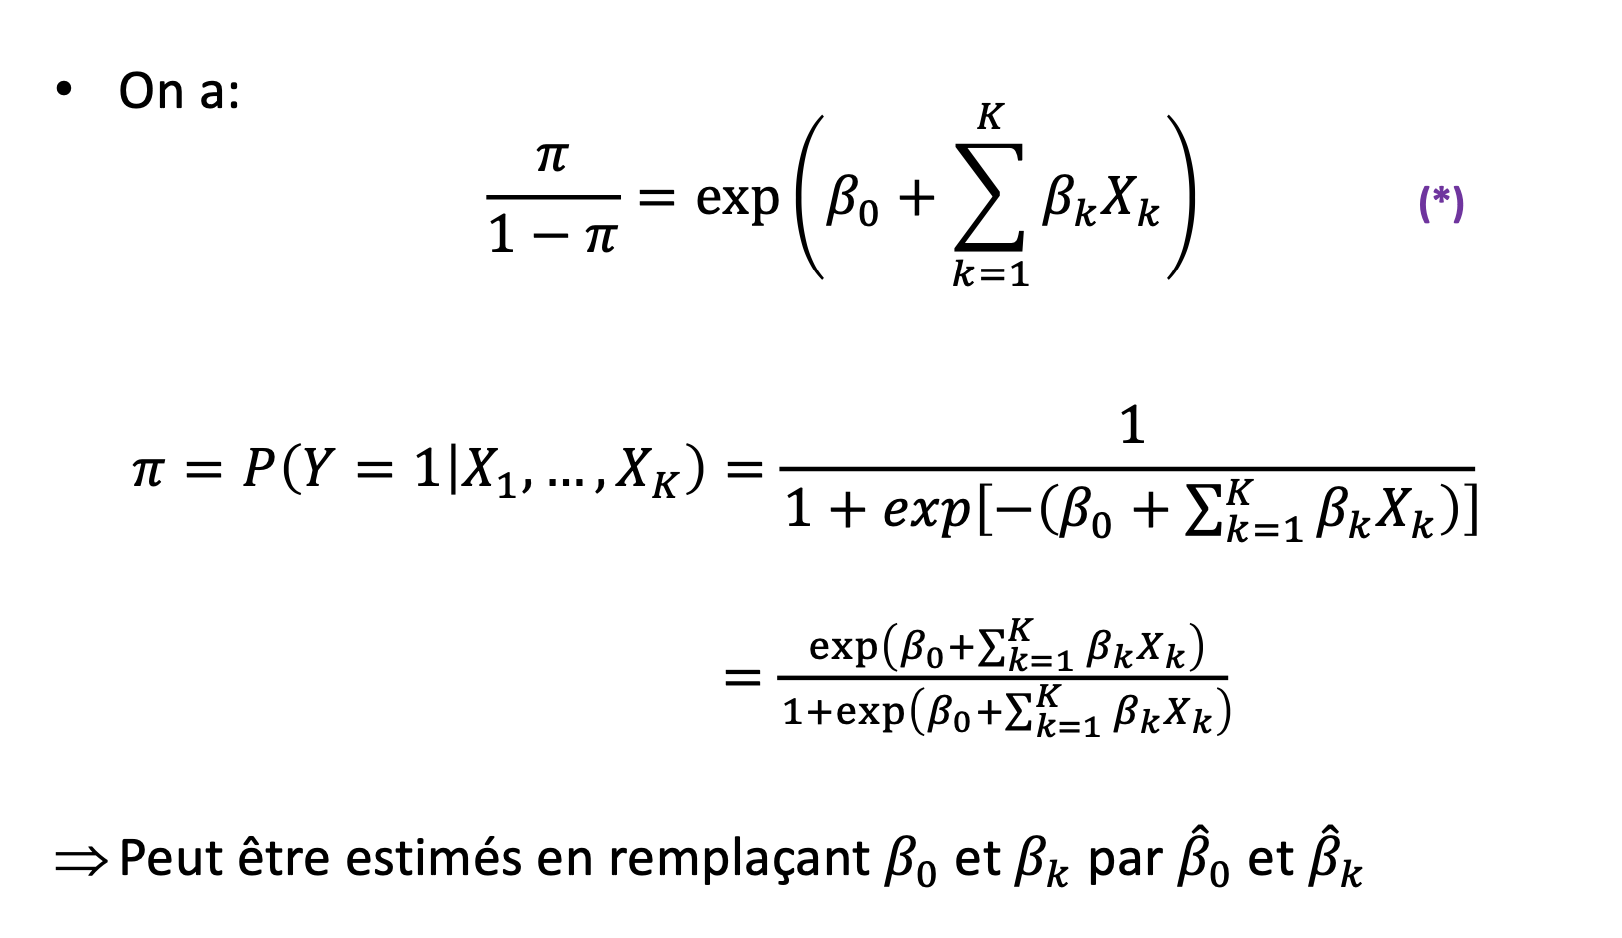
\includegraphics[scale=0.5]{images/pi_logit.png}
    \caption{Valeur de \pi pour logit régression}
    \label{fig:my_label}
\end{figure}

\begin{figure}[H]
    \centering
    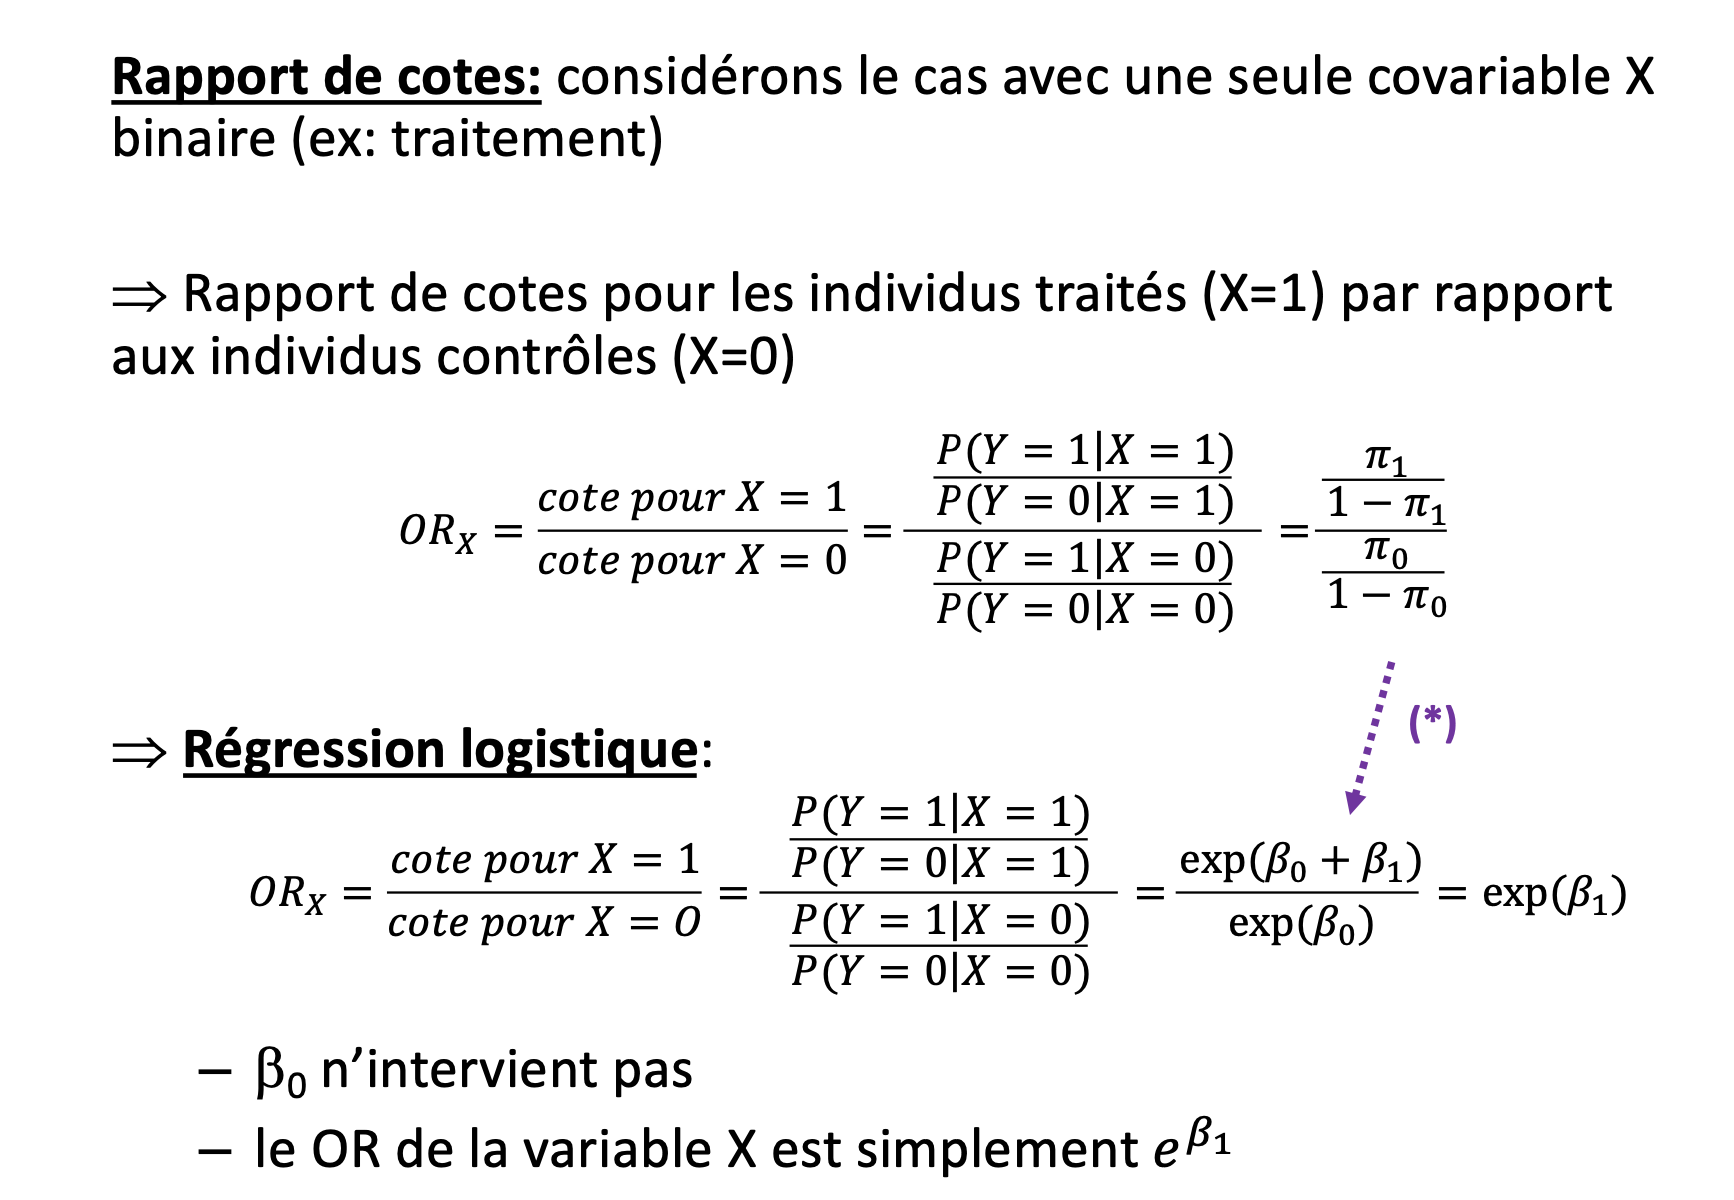
\includegraphics[scale=0.5]{images/rapportcote_logit.png}
    \caption{rapport des cotes en logit régression}
    \label{fig:my_label}
\end{figure}

\subsubsection{Estimation des paramètres}
L’estimation des paramètres peut se faire en appliquant le principe du maximum de vraisemblance. 
\begin{figure}[H]
    \centering
    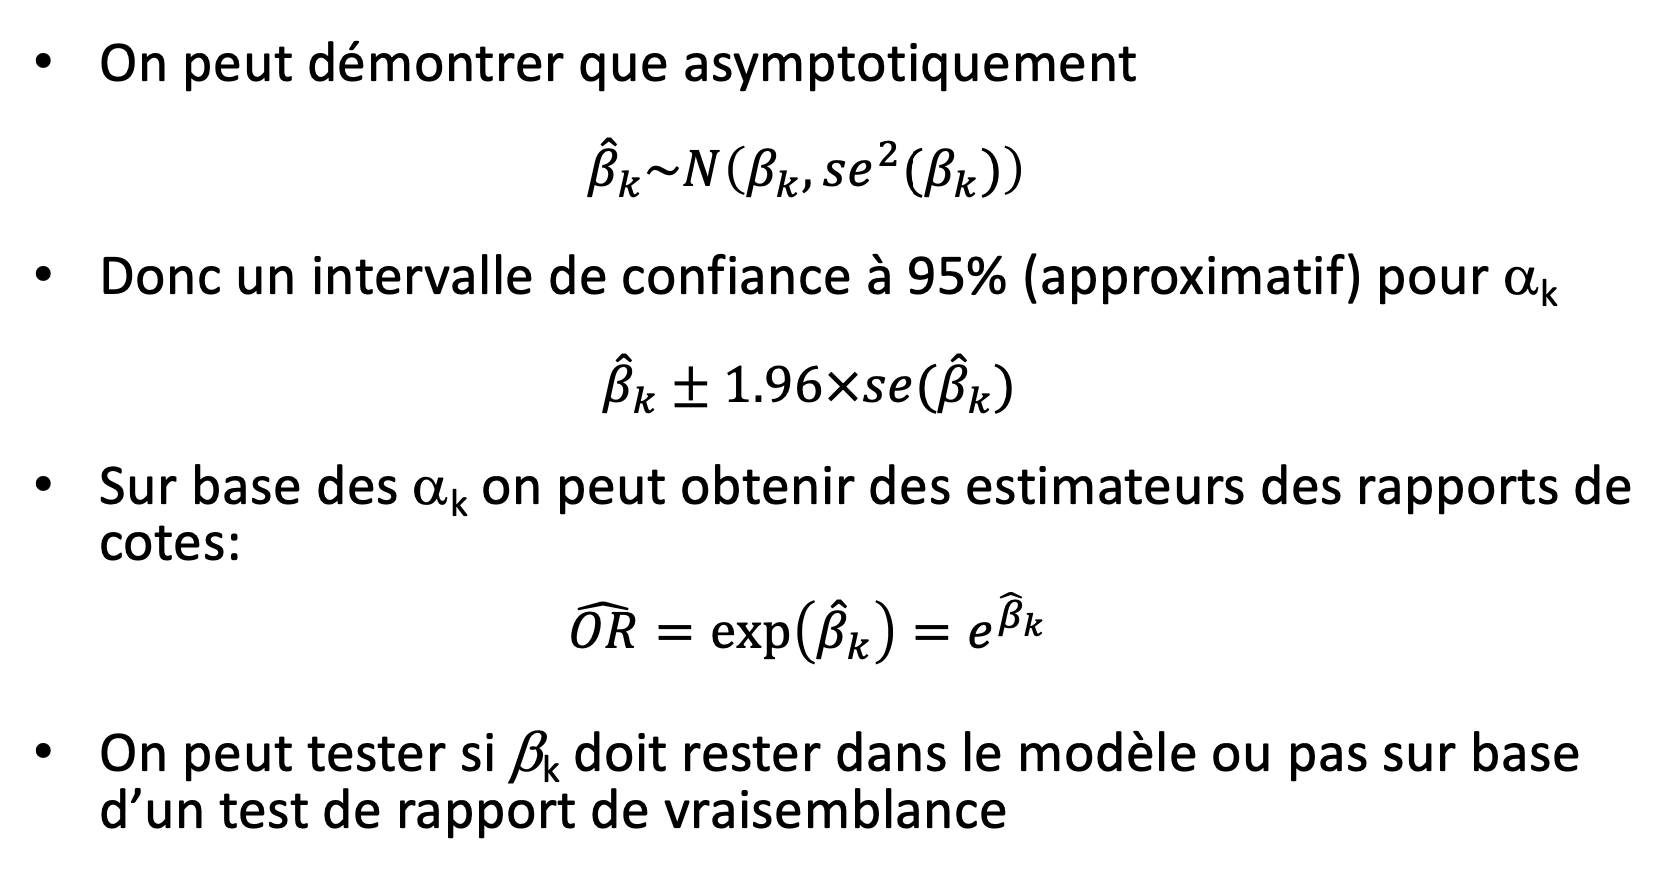
\includegraphics[scale =0.5]{images/estimation_logit.png}
    \caption{estimation des paramètres pour logit régression}
    \label{fig:my_label}
\end{figure}
\subsubsection{Test du maximum de vraisemblance}

\begin{figure}[H]
    \centering
    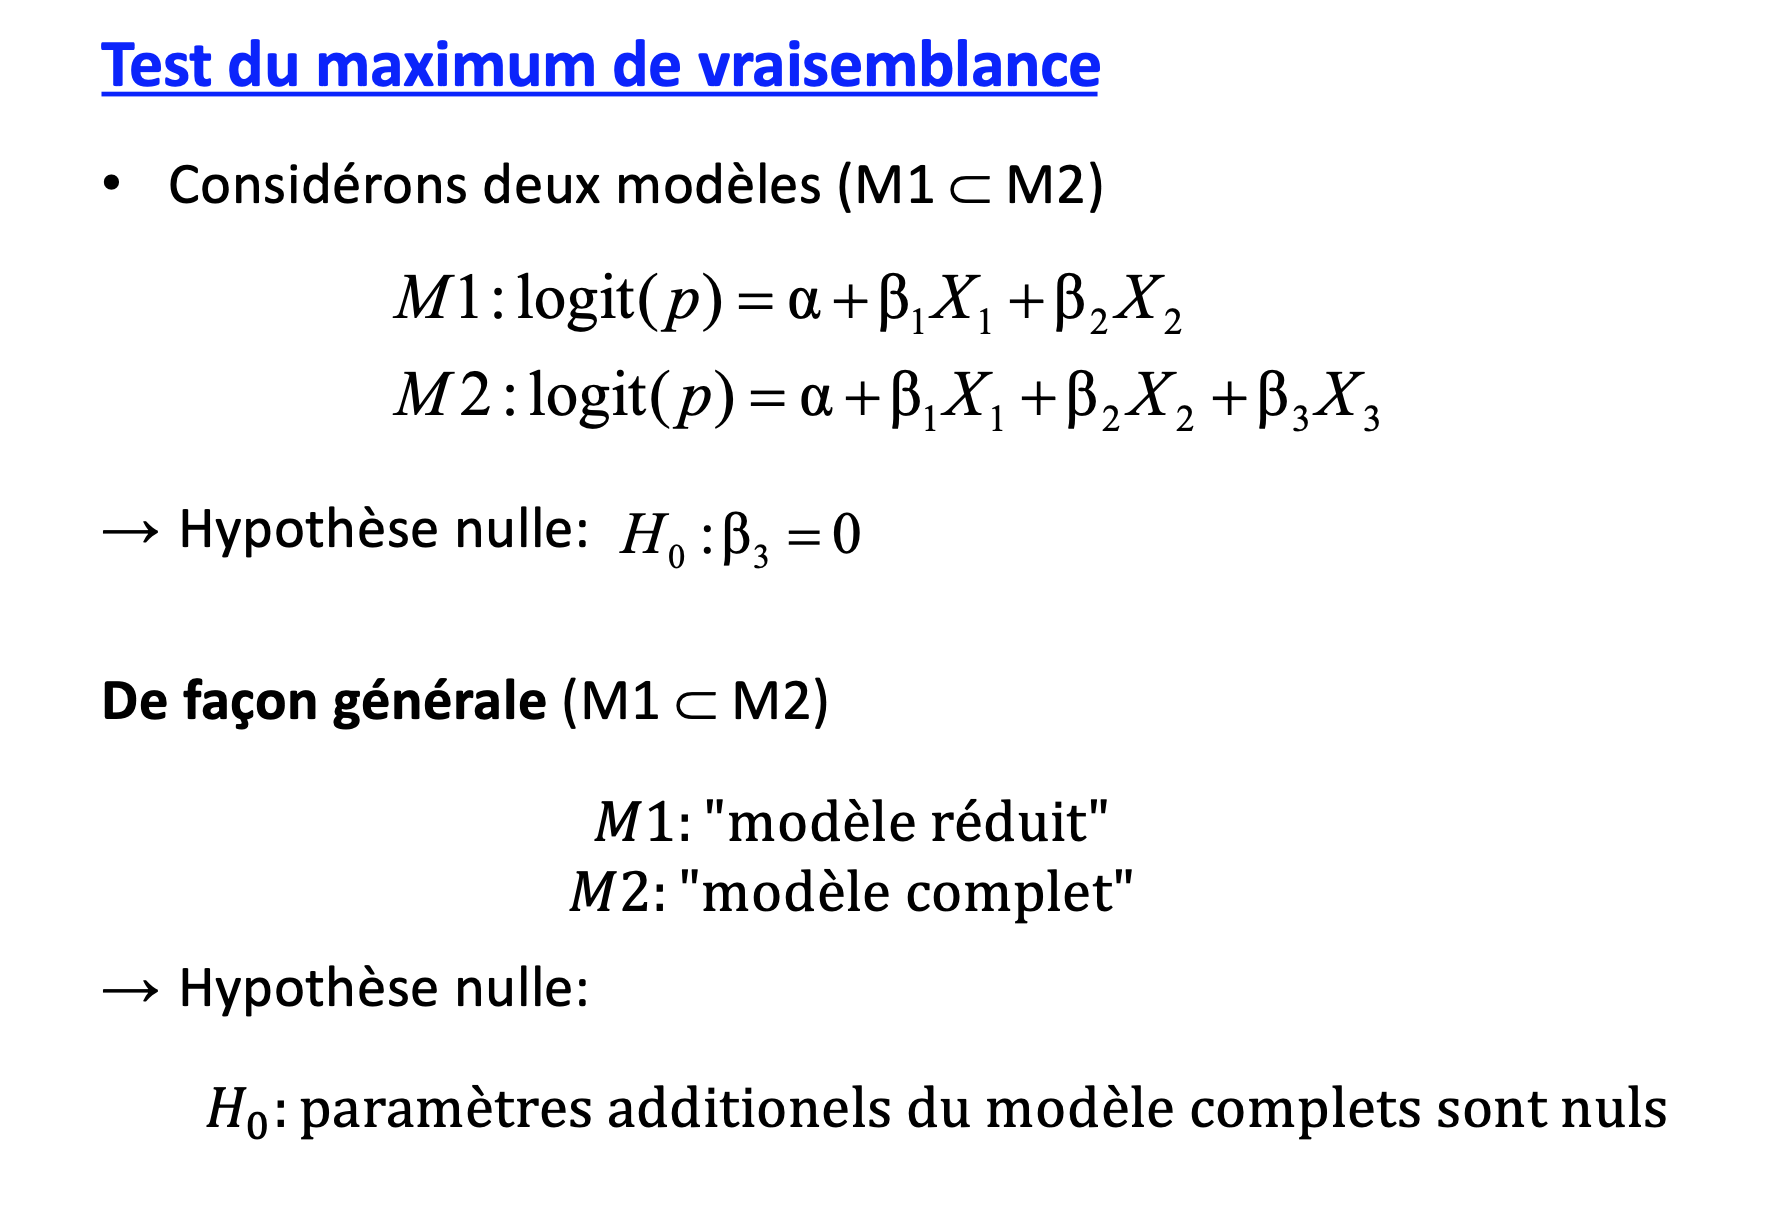
\includegraphics[scale = 0.5]{images/test_vraisemblance.png}
    \caption{Test du maximum de vraisemblance}
    \label{fig:my_label}
\end{figure}
\subsubsection{Test de Wald}
\begin{figure}[H]
    \centering
    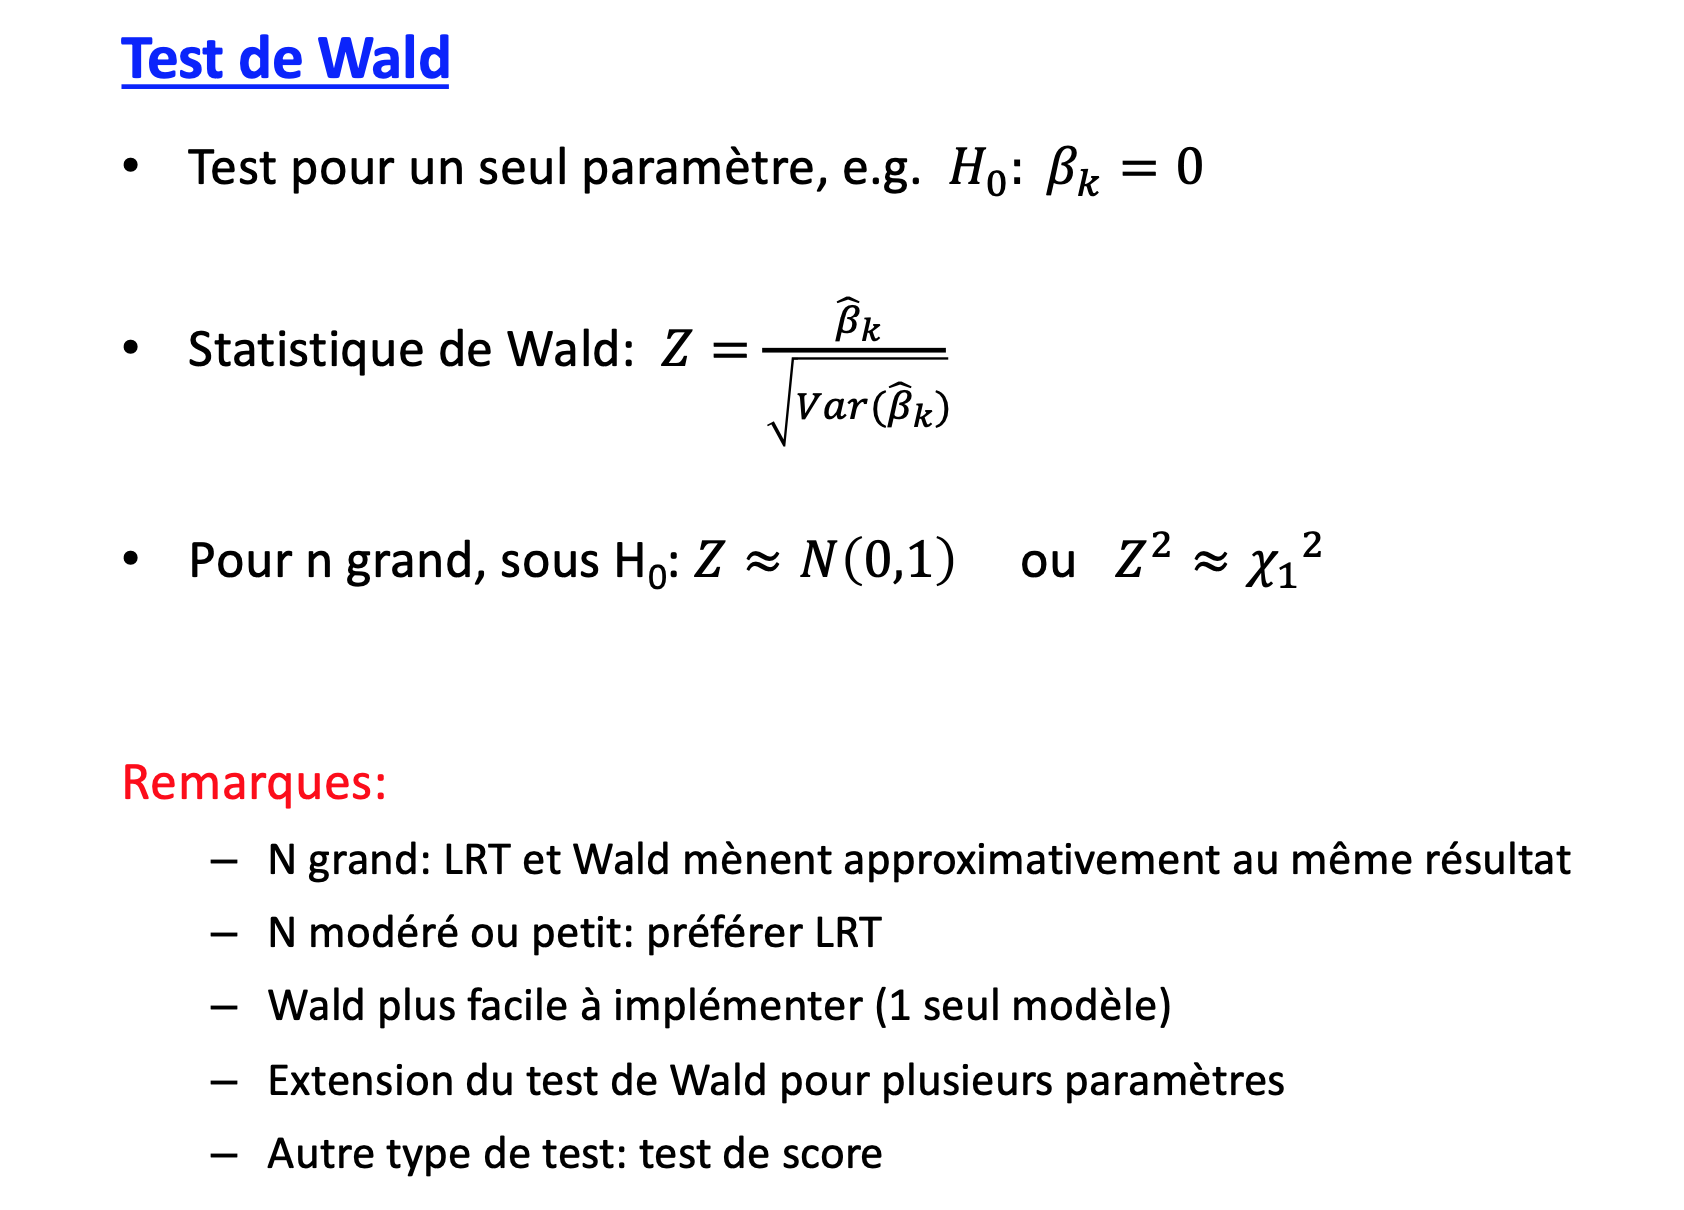
\includegraphics[scale = 0.5]{images/test_wald.png}
    \caption{Test de Wald}
    \label{fig:my_label}
\end{figure}
\subsection{Cas de plus de 2 groupes de traitement}
Soit, on peut faire une Comparaison globale et cela revient à une généralisation directe du test chi-carré pour une table de contingence $r×c$. Soit, on fait des comparaisons deux à deux mais cela implique un problème de multiplicité de test. Le même type de solutions que précédemment peut être utilisé. 

\section{Endpoint de survie}
Pour chaque patient : temps entre une origine et un événement prédéfini (exemple survie). On a une variable continue positive. Mais Au moment de la fin de l'étude, l'événement d'intérêt n'est généralement pas observé pour tous les patients. On parle dans ce cas-là de \textbf{données censurées (à droite)}. Il faut faire attention que ce processus de censure doit être indépendant de l'apparition des événements analysés (donc une censure administrative, c'est ok).


\subsection{Résumer des données de survie}
Méthodes "classiques" (moyenne, histogrammes, …) ne
fonctionnent pas (à cause de la censure !)\\
On peut utiliser une fonction de survie : 
$$S(t) = P(T>t)$$
$S(t)$ représente pour chaque instant t la probabilité que le temps jusqu'à l'événement soit le plus grand que cet instant. On va utiliser une représentation graphique de l'estimateur de la fonction de survie= \textbf{Estimateur de Kaplan-Meier} qui se calcule de la manière suivante :
$$\widehat{S}(t) = \prod_{j=0}^t (1-\frac{O_{j}}{n_{j}})$$
Un exemple est donné dans les slides.

\subsection{Effet traitement}
Pour mesurer l'effet d'un traitement, on va utiliser les éléments suivants.
\subsubsection{Test du Logrank}
On va comparer les courbes de survie pour 2 groupes.
On définit :
\begin{itemize}
    \item Groupe 1 = groupe expérimental $S_{exp}(t)$
    \item Groupe 2 = groupe standard $S_{std}(t)$
\end{itemize}
On va avoir comme test d'hypothèse :
\begin{figure}[H]
    \centering
    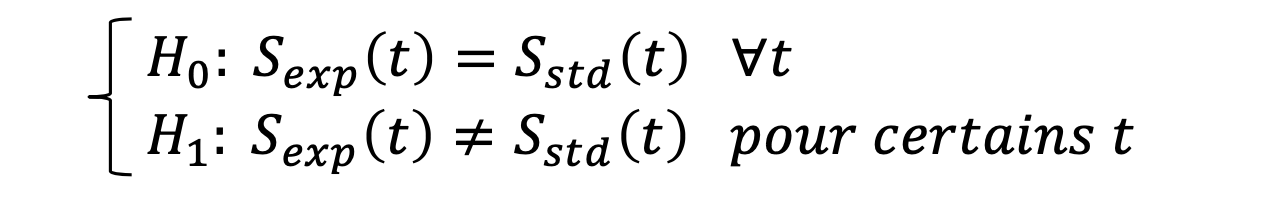
\includegraphics[scale = 0.5]{images/logrank.png}
    \caption{test d'hypothèse pour un test du Longrank}
    \label{fig:my_label}
\end{figure}

\subsection{Hazards ratio (HR)}
Cela permet d'estimer le rapport de risques d'événement entre deux groupes. 
\begin{figure}[H]
    \centering
    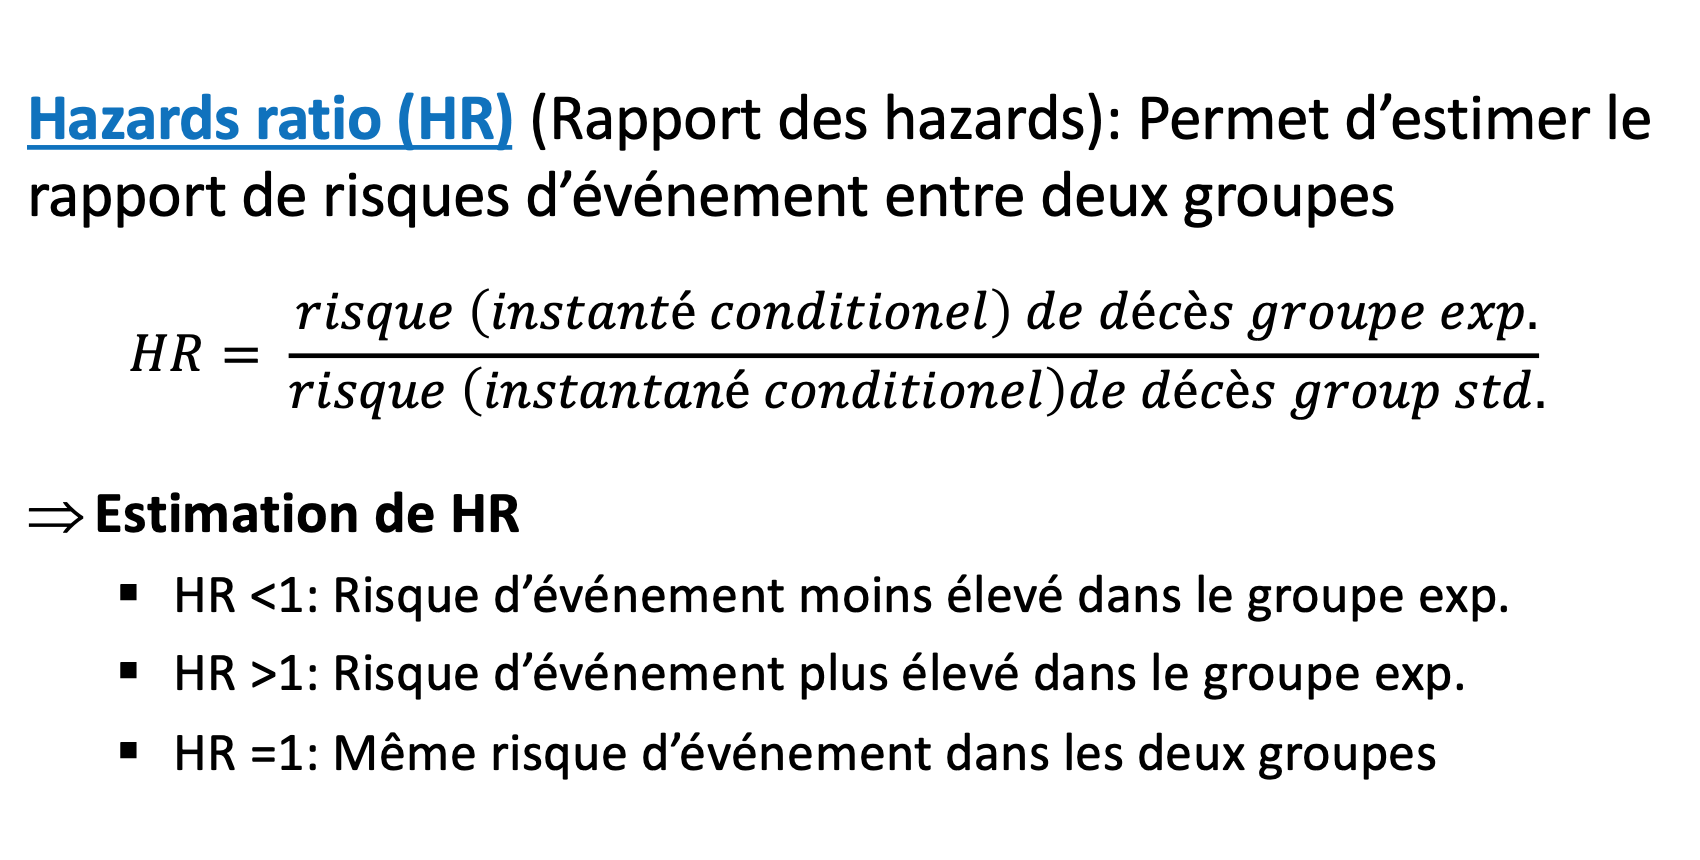
\includegraphics[scale=0.5]{images/hazardratio.png}
    \caption{Hazard ratio (HR)}
    \label{fig:my_label}
\end{figure}

\subsection{Modélisation des données de survie}
Il existe plusieurs modèles de régression s’appliquant aux données de survie, le plus connu est le modèle de Cox (modèle de hazards proportionnels).

\subsection{Modèle de Cox}
Modèle semi-paramétrique, car on a un terme qui dépend que du temps et l'autre des paramètres.
\begin{figure}[H]
    \centering
    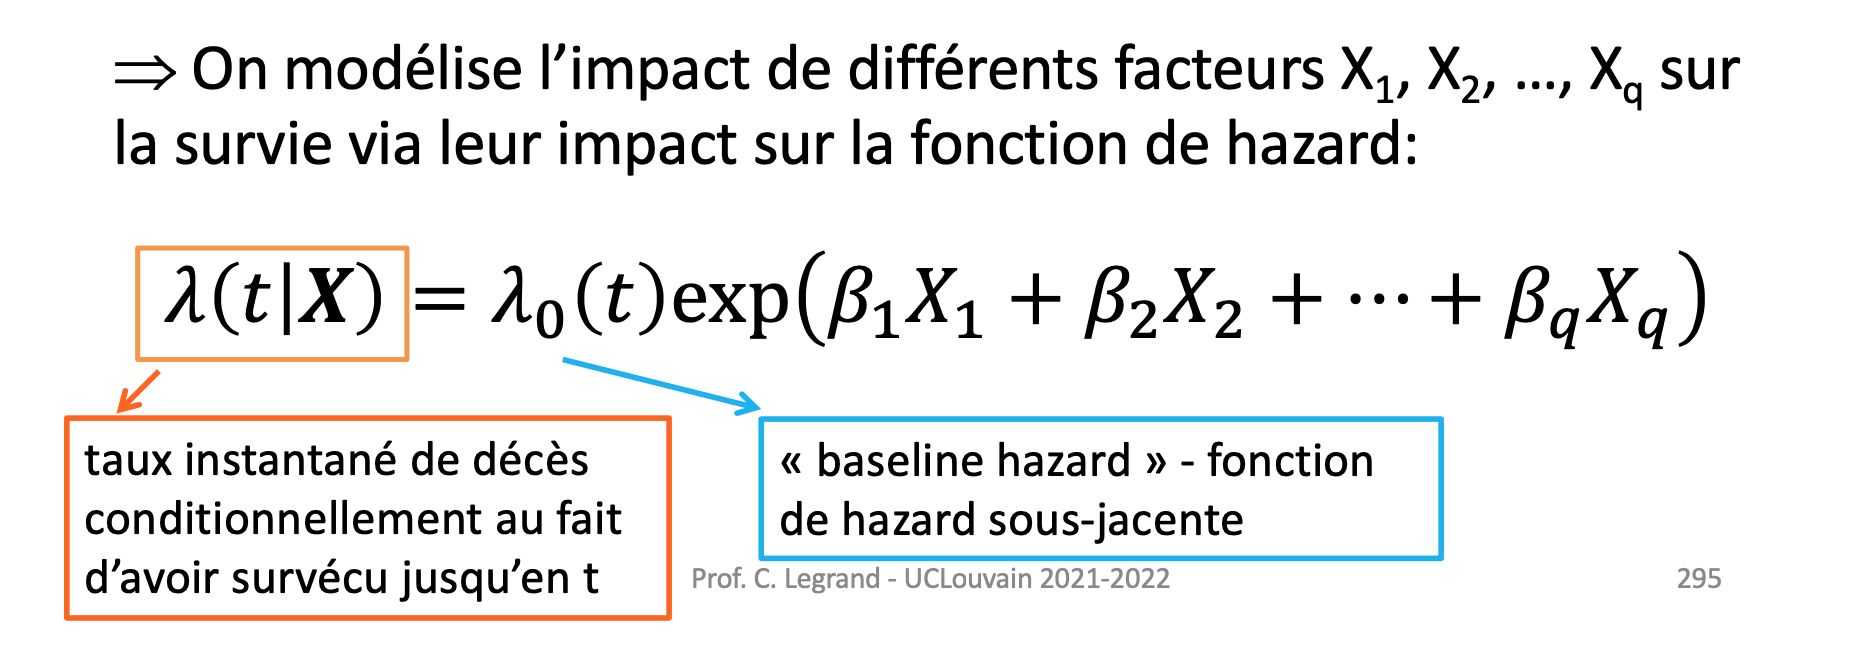
\includegraphics[scale=0.5]{images/modelecox.png}
    \caption{modèle de Cox}
    \label{fig:my_label}
\end{figure}

Quelques résultats importants :

\begin{figure}[H]
    \centering
    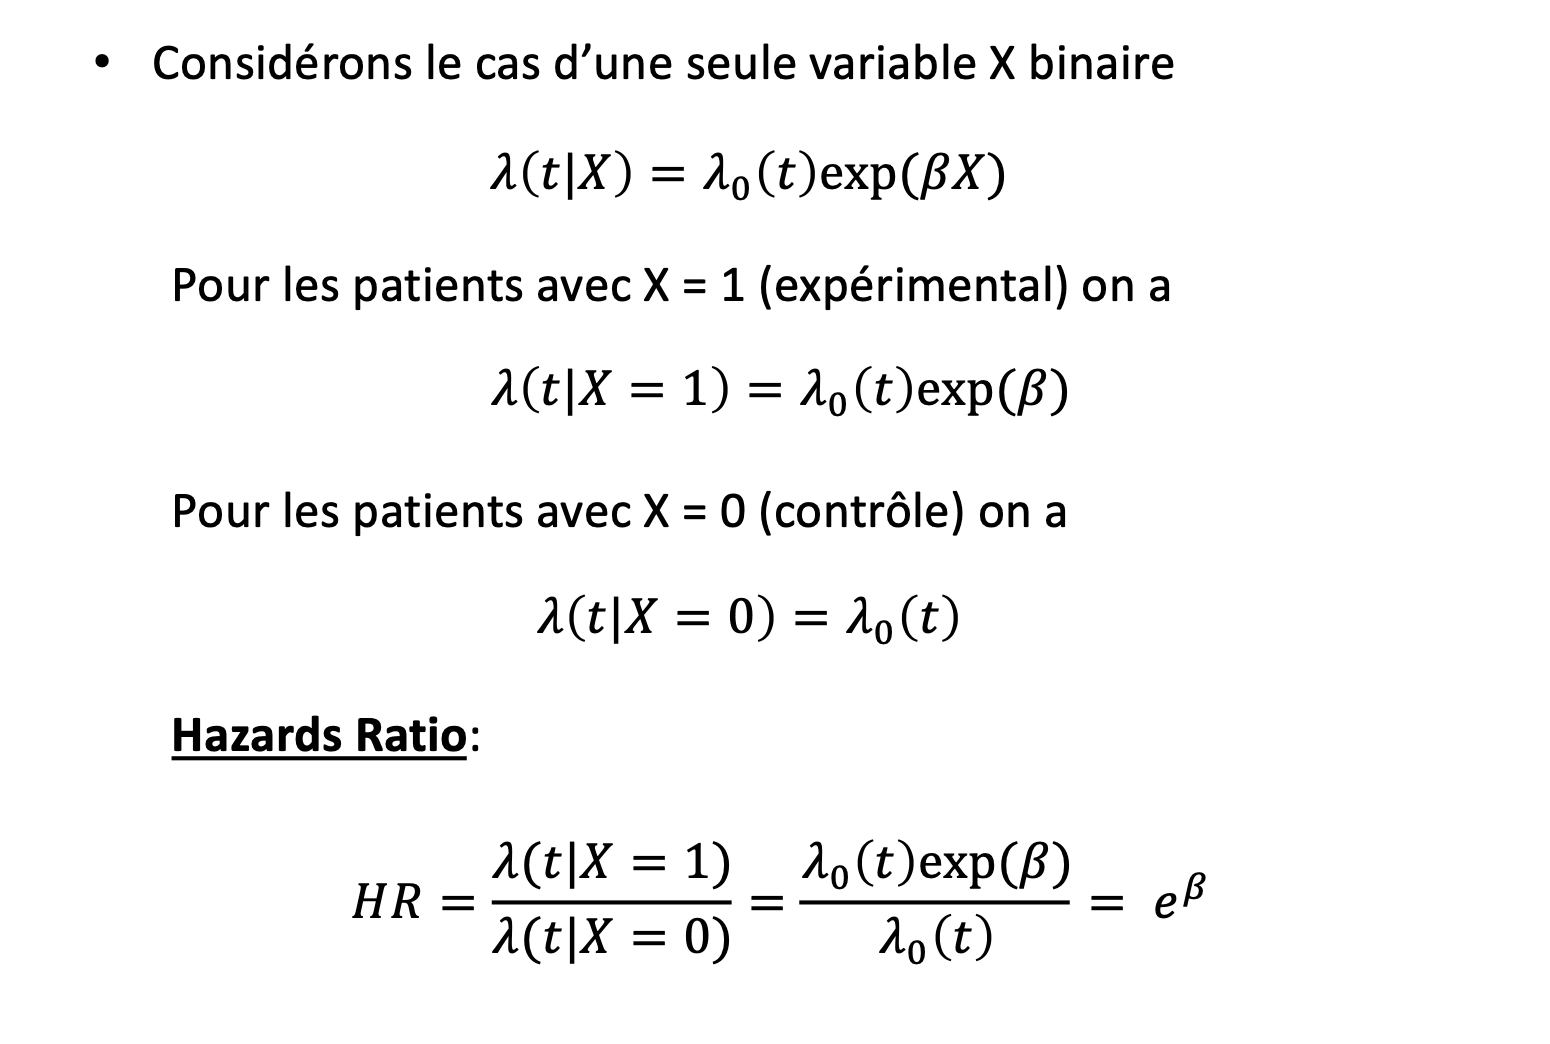
\includegraphics[scale=0.5]{images/cox_1.png}
    \caption{Résultat avec modèle de Cox}
    \label{fig:my_label}
\end{figure}

\begin{figure}[H]
    \centering
    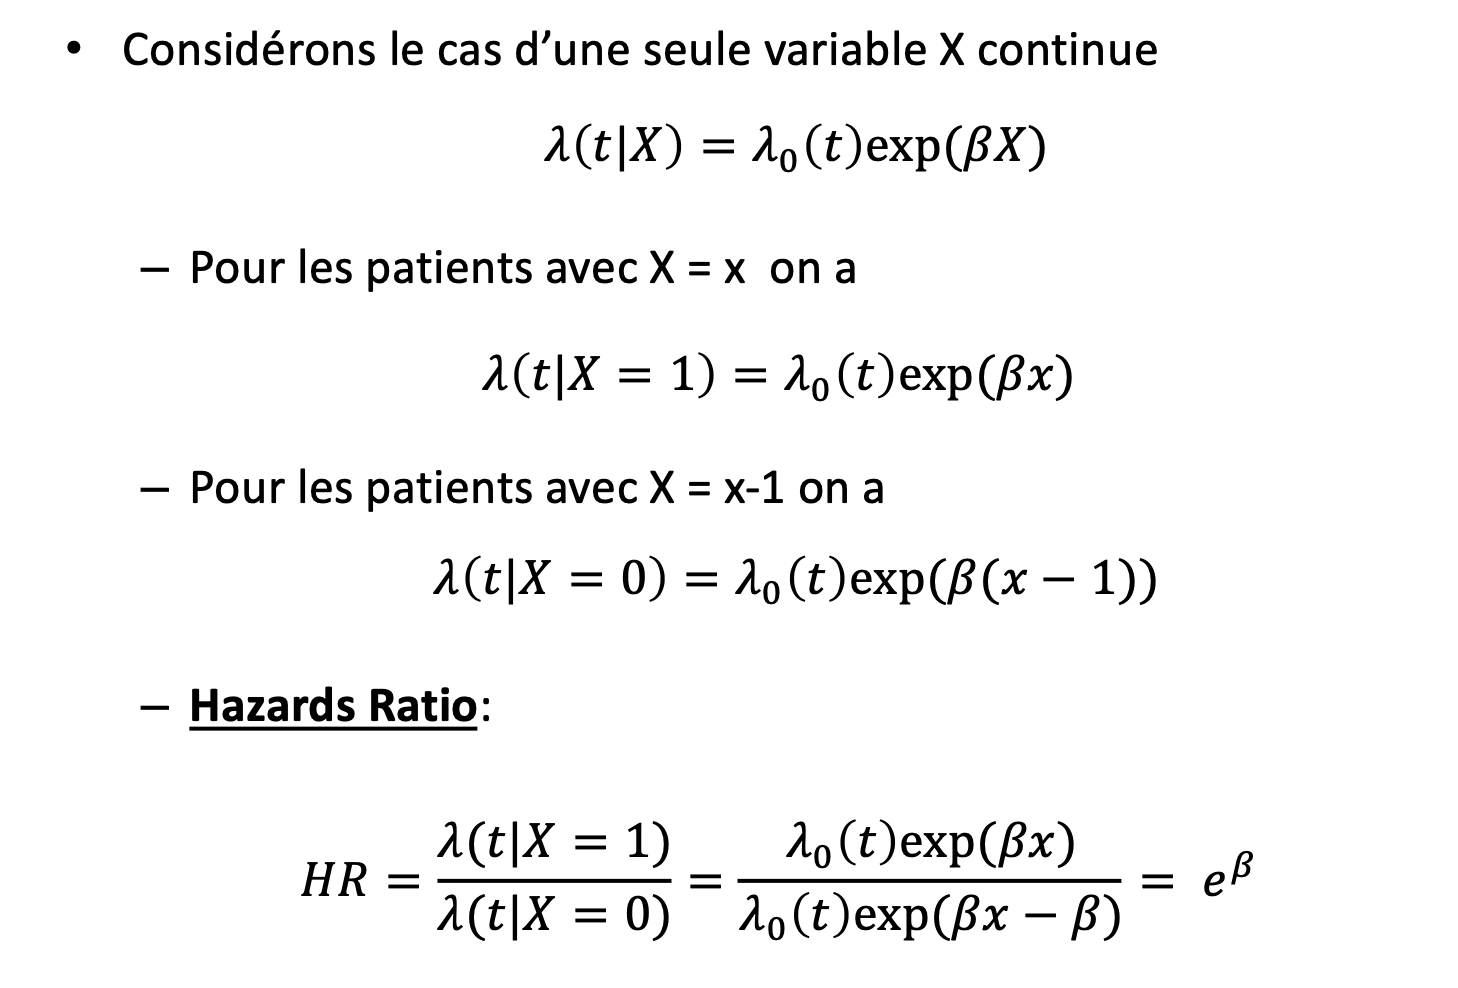
\includegraphics[scale=0.5]{images/cox_2.png}
    \caption{Résultat avec modèle de Cox}
    \label{fig:my_label}
\end{figure}

\begin{figure}[H]
    \centering
    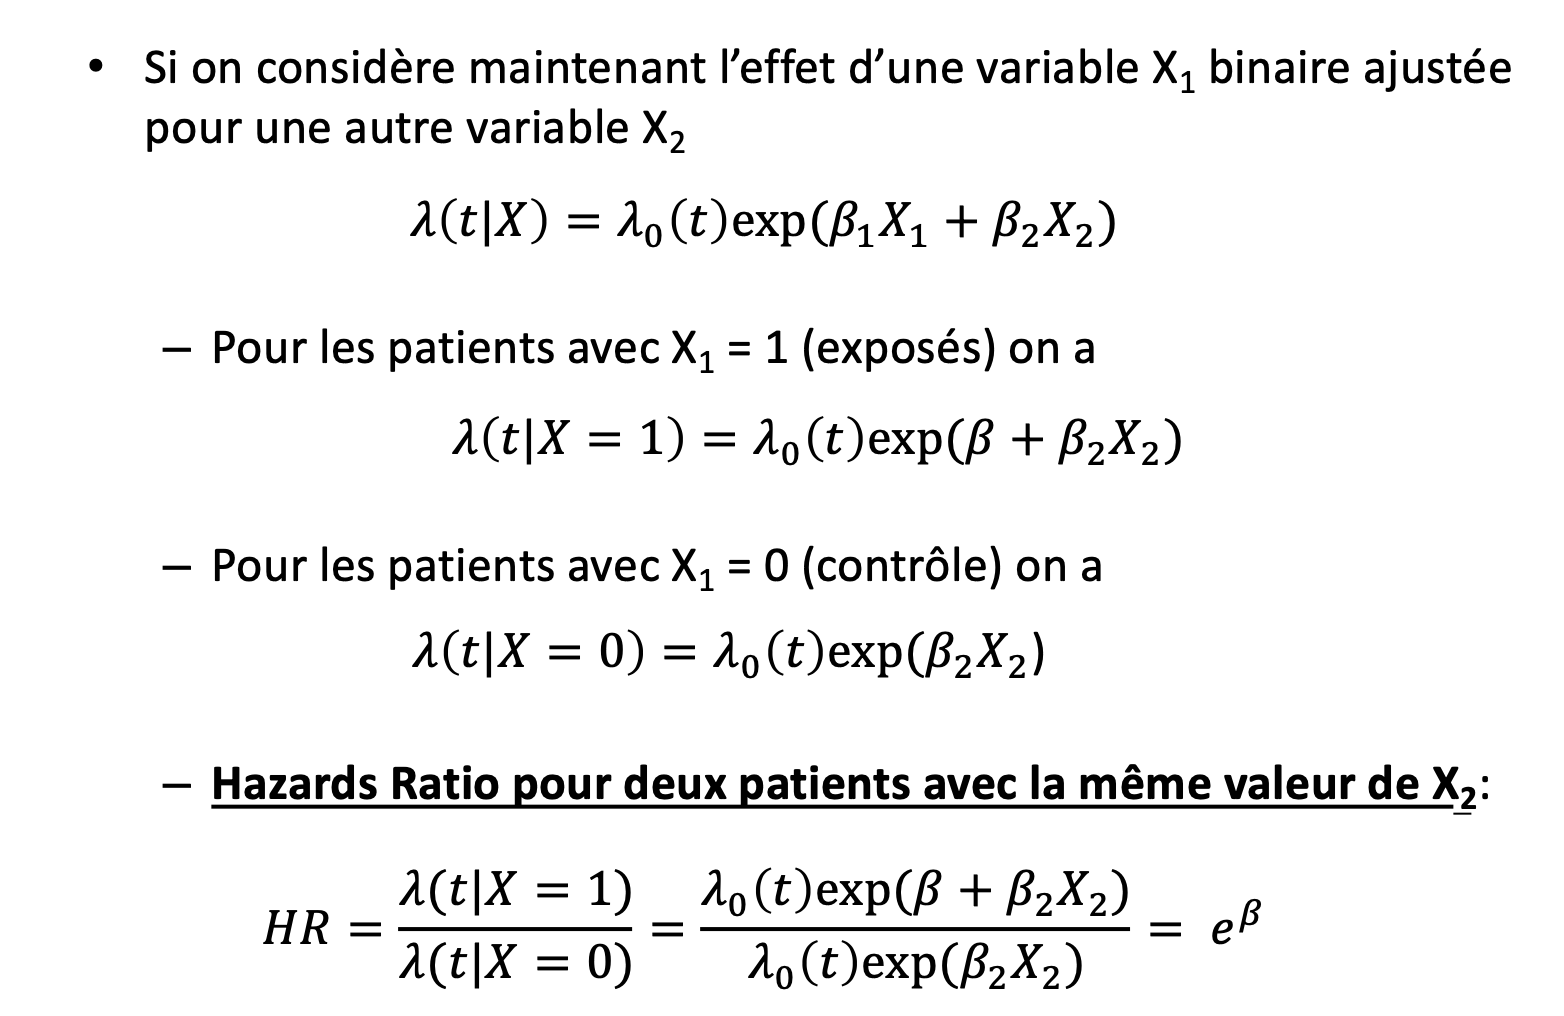
\includegraphics[scale=0.5]{images/cox_3.png}
    \caption{Résultat avec modèle de Cox}
    \label{fig:my_label}
\end{figure}

\subsection{Code R}
voir slides

